% Created 2019-03-14 Thu 11:48
% Intended LaTeX compiler: pdflatex
\documentclass[a4paper, 12pt]{article}
\usepackage[utf8]{inputenc}
\usepackage[T1]{fontenc}
\usepackage{graphicx}
\usepackage{grffile}
\usepackage{longtable}
\usepackage{wrapfig}
\usepackage{rotating}
\usepackage[normalem]{ulem}
\usepackage{amsmath}
\usepackage{textcomp}
\usepackage{amssymb}
\usepackage{capt-of}
\usepackage{hyperref}
\usepackage[left=2.5cm, right=2.5cm, top=2.5cm, bottom=2.5cm, bindingoffset=1.5cm, head=15pt]{geometry}
\usepackage{setspace}
\usepackage{caption}
\onehalfspacing
\usepackage[official]{eurosym}
\usepackage{amsmath}
\usepackage{amssymb}
\usepackage{notation/rl}
\usepackage{notation/model}
\usepackage{template/informs}
\let\enumerate\henumerate
\let\itemize\hitemize
\usepackage{fancyhdr}
\pagestyle{fancy}
\fancyhead{}
\fancyfoot{}
\fancyhead[LE,RO]{\textsl{\leftmark}}
\fancyhead[RE,LO]{Tobias Richter}
\fancyfoot[C]{\thepage}
\renewcommand{\headrulewidth}{0.4pt}
\renewcommand{\footrulewidth}{0pt}
\usepackage{apacite}
\let\cite\shortcite
\let\textcite\shortciteA
\usepackage[nohyperlinks]{acronym}
\interfootnotelinepenalty=10000
\usepackage[notlof,notlot,nottoc]{tocbibind}
\newcommand{\studentID}{558305}
\newcommand{\thesistype}{Master Thesis}
\newcommand{\supervisor}{Univ.-Prof. Dr. Wolfgang Ketter}
\newcommand{\cosupervisor}{Karsten Schroer}
\pagenumbering{Roman}
\author{Tobias Richter}
\date{\today}
\title{Reinforcement Learning Portfolio Optimization of Electric Vehicle Virtual Power Plants}
\hypersetup{
 pdfauthor={Tobias Richter},
 pdftitle={Reinforcement Learning Portfolio Optimization of Electric Vehicle Virtual Power Plants},
 pdfkeywords={},
 pdfsubject={},
 pdfcreator={Emacs 26.1 (Org mode 9.2.1)},
 pdflang={English}}
\begin{document}

\makeatletter
\begin{titlepage}
    \begin{center}
        \vspace*{1cm}

        \Large
        \textbf{\@title{}}

        \vspace{1.5cm}

        \thesistype{}

        \vspace{1cm}

        \begin{figure}[htbp]
             \centering
             
\includegraphics[width=.5\linewidth]{./fig/UoC_Logo.png}
        \end{figure}

        \vspace{1cm}

        \large
        \textbf{Author}: \@author{} (Student ID: \studentID{})\\
        \large
        \textbf{Supervisor}: \supervisor{}\\
        \large
        \textbf{Co-Supervisor}: \cosupervisor{}

        \vspace{1cm}
        \large
        Department of Information Systems for Sustainable Society\\
        Faculty of Management, Economics and Social Sciences\\
        University of Cologne\\

        \vspace{1cm}
        \@date{}

    \end{center}
\end{titlepage}
\makeatother
\clearpage
\thispagestyle{empty}
\section*{Eidesstattliche Versicherung}
\label{sec:SOOA}

\vspace{2.5cm}

% Statement of original authorship - Needs to be in German
% see also here: https://www.wiso.uni-koeln.de/sites/fakultaet/dokumente/PA/formulare/eidesstattliche_erklaerung.pdf

Hiermit versichere ich an Eides statt, dass ich die vorliegende Arbeit selbstständig und ohne die Benutzung anderer als der angegebenen Hilfsmittel angefertigt habe. Alle Stellen, die wörtlich oder sinngemäß aus veröffentlichten und nicht veröffentlichten Schriften entnommen wurden, sind als solche kenntlich gemacht. Die Arbeit ist in gleicher oder ähnlicher Form oder auszugsweise im Rahmen einer anderen Prüfung noch nicht vorgelegt worden. Ich versichere, dass die eingereichte elektronische Fassung der eingereichten Druckfassung vollständig entspricht.

\vspace{1cm}

\noindent
Die Strafbarkeit einer falschen eidesstattlichen Versicherung ist mir bekannt, namentlich die Strafandrohung gemäß § 156 StGB bis zu drei Jahren Freiheitsstrafe oder Geldstrafe bei vorsätzlicher Begehung der Tat bzw. gemäß § 161 Abs. 1 StGB bis zu einem Jahr Freiheitsstrafe oder Geldstrafe bei fahrlässiger Begehung.

\vspace{3cm}
\noindent
\textbf{Tobias Richter}

\vspace{0.5cm}
\noindent
Köln, den 01.05.2019
\clearpage

\setcounter{page}{1}
\tableofcontents
\clearpage
\listoffigures
\clearpage
\listoftables
\clearpage

\section*{List of Abbreviations} \markboth{LIST OF ABBREVIATIONS}{}
\begin{acronym}[GCRM]
	\acro{ANN}{Artificial Neural Network}
	\acro{DP}{Dynamic Programming}
	\acro{DSO}{Distribution System Operator}
	\acro{EPEX}{European Power Exchange}
	\acro{EV}{Electric Vehicle}
	\acro{GCRM}{German Control Reserve Market}
	\acro{GP}{Genetic Programming}
	\acro{MAW}{Mean Asymmetric Weighted Objective Function}
	\acro{MC}{Monte Carlo}
	\acro{MDP}{Markov Decision Process}
	\acro{PDF}{Probability Density Function}
	\acro{RES}{Renewable Energy Sources}
	\acro{RL}{Reinforcement Learning}
	\acro{TD}{Temporal-Difference}
	\acro{TSO}{Transmission System Operator}
	\acro{V2G}{Vehicle-to-Grid}
	\acro{VPP}{Virtual Power Plant}
\end{acronym}
\clearpage
\section*{Summary of Notation} \markboth{SUMMARY OF NOTATION}{}
Capital letters are used for random variables, whereas lower case letters are used for
the values of random variables and for scalar functions. Quantities that are required to
be real-valued vectors are written in bold and in lower case (even if random variables).
\begin{tabbing}
    \=~~~~~~~~~~~~~~~~~~  \= \kill
    \>$\defeq$            \> equality relationship that is true by definition\\
    \>$\approx$           \> approximately equal\\
    \>$\E{X}$             \> expectation of a random variable $X$, i.e., $\E{X}\defeq\sum_x p(x)x$\\
    \>$\Re$               \> set of real numbers\\
    \>$\leftarrow$        \> assignment\\
    \\
    \>$\e$                \> probability of taking a random action in an \e-greedy policy\\
    \>$\alpha$            \> step-size parameter\\
    \>$\gamma$            \> discount-rate parameter\\
    \>$\lambda$           \> decay-rate parameter for eligibility traces\\
    \\
    \>$s, s'$             \> states\\
    \>$a$                 \> an action\\
    \>$r$                 \> a reward\\
    \>$\S$                \> set of all nonterminal states\\
    \>$\A$                \> set of all available actions\\
    \>$\R$                \> set of all possible rewards, a finite subset of $\Re$\\
    \>$\subset$           \> subset of; e.g., $\R\subset\Re$\\
    \>$\in$               \> is an element of; e.g., $s\in\S$, $r\in\R$\\
    \\
    \>$t$                 \> discrete time step\\
    \>$T, T(t)$           \> final time step of an episode, or of the episode including time step $t$\\
    \>$A_t$               \> action at time $t$\\
    \>$S_t$               \> state at time $t$, typically due, stochastically, to $S_{t-1}$ and $A_{t-1}$\\
    \>$R_t$               \> reward at time $t$, typically due, stochastically, to $S_{t-1}$ and $A_{t-1}$\\
    \>$\pi$               \> policy (decision-making rule)\\
    \>$\pi(s)$            \> action taken in state $s$ under {\it deterministic\/} policy $\pi$\\
    \>$\pi(a|s)$          \> probability of taking action $a$ in state $s$ under {\it stochastic\/} policy $\pi$\\
    \>$G_t$               \> return following time $t$\\
    \\
    \>$\p(s',r|s,a)$      \> probability of transition to state $s'$ with reward $r$, from state $s$ and action $a$\\
    \>$\p(s'|s,a)$        \> probability of transition to state $s'$, from state $s$ taking action $a$\\
    \>$\vpi(s)$           \> value of state $s$ under policy $\pi$ (expected return)\\
    \>$\vstar(s)$         \> value of state $s$ under the optimal policy\\
    \>$\qpi(s,a)$         \> value of taking action $a$ in state $s$ under policy $\pi$\\
    \>$\qstar(s,a)$       \> value of taking action $a$ in state $s$ under the optimal policy\\
    \>$V, V_t$            \> array estimates of state-value function $\vpi$ or $\vstar$\\
    \>$Q, Q_t$            \> array estimates of action-value function $\qpi$ or $\qstar$\\
    \\
    \>$d$                 \> dimensionality---the number of components of $\w$\\
    \>$\w$                \> $d$-vector of weights underlying an approximate value function\\
    \>$\hat v(s,\w)$      \> approximate value of state $s$ given weight vector $\w$\\
    \>$\mu(s)$            \> on-policy distribution over states\\
    \>$\MSVEm$            \> mean square value error\\
\end{tabbing}
\clearpage

\pagenumbering{arabic}

\section{Introduction}
\label{sec:orgd67fe5f}
\subsection{Research Motivation}
\label{sec:orgf35b784}
\begin{itemize}
\item \cite{lopes11_integ_elect_vehic_elect_power_system}
\end{itemize}
\subsection{Research Question}
\label{sec:org1eeb320}
\subsection{Relevance}
\label{sec:org04868e2}

\section{Background}
\label{sec:orga59649b}
\subsection{Smart Electricity Markets}
\label{sec:org85090bf}
On electricity markets, actors participate in auctions to match the supply of
electricity generation and the demand for electricity consumption. Participants
place asks (sale offers) and bids (purchase orders). The electricity price is
determined by an auction mechanism, which can take different forms depending on
the type of market. Germany, like many other western countries, has a
liberalized energy system in which the generation and distribution of
electricity are decoupled. Multiple electricity markets exist in a liberalized
energy system. They differ in the auction design and in their reaction time
between the order contract and the delivery of electricity. Day-ahead markets
and spot markets have a reaction time between a day and several hours, whereas
in operating reserve markets the reaction time ranges from minutes to seconds.
The auction mechanism design is essential for electricity markets
\cite{kambil98_reeng_dutch_flower_auction}. Electricity markets work according to
the merit order principle in which resources are considered in ascending order
of the energy price until the capacity demand is met. The clearing price is
determined by the energy price, at the point where supply meets demand. Payment
models differ in the markets: In contrast to day-ahead markets, where a uniform
pricing schema is applied, in secondary reserve markets and intraday markets
bidders, get compensated by the price they bid (pay-as-bid principle).

EV fleet operators can offer the capacity of their EV batteries on multiple
markets at the same time to make use of the different market properties. On
operating reserve markets,prices are usually more volatile and consequently more
attractive for VPPs \cite{tomic07_using_fleet_elect_drive_vehic_grid_suppor}.
Operating reserve markets also bear a higher risk for the fleet: Commitments
have to be made one week in advance when customer demands are still uncertain.
In order to not face penalties for unfulfilled commitments only a conservative
amount of capacity can be offered to the market. On the other hand, spot markets
allow participants to continuously trade electricity products up to five minutes
prior to delivery. At this point in time, it is possible to predict available
battery capacity of the fleet with high accuracy. This certainty creates the
possibility to trade the remaining available capacity with low risk at the spot
market. In the following, we will explain the market design of balancing markets
and spot markets in more detail, since they are the markets we included in our
research.

\begin{figure}[htbp]
\centering
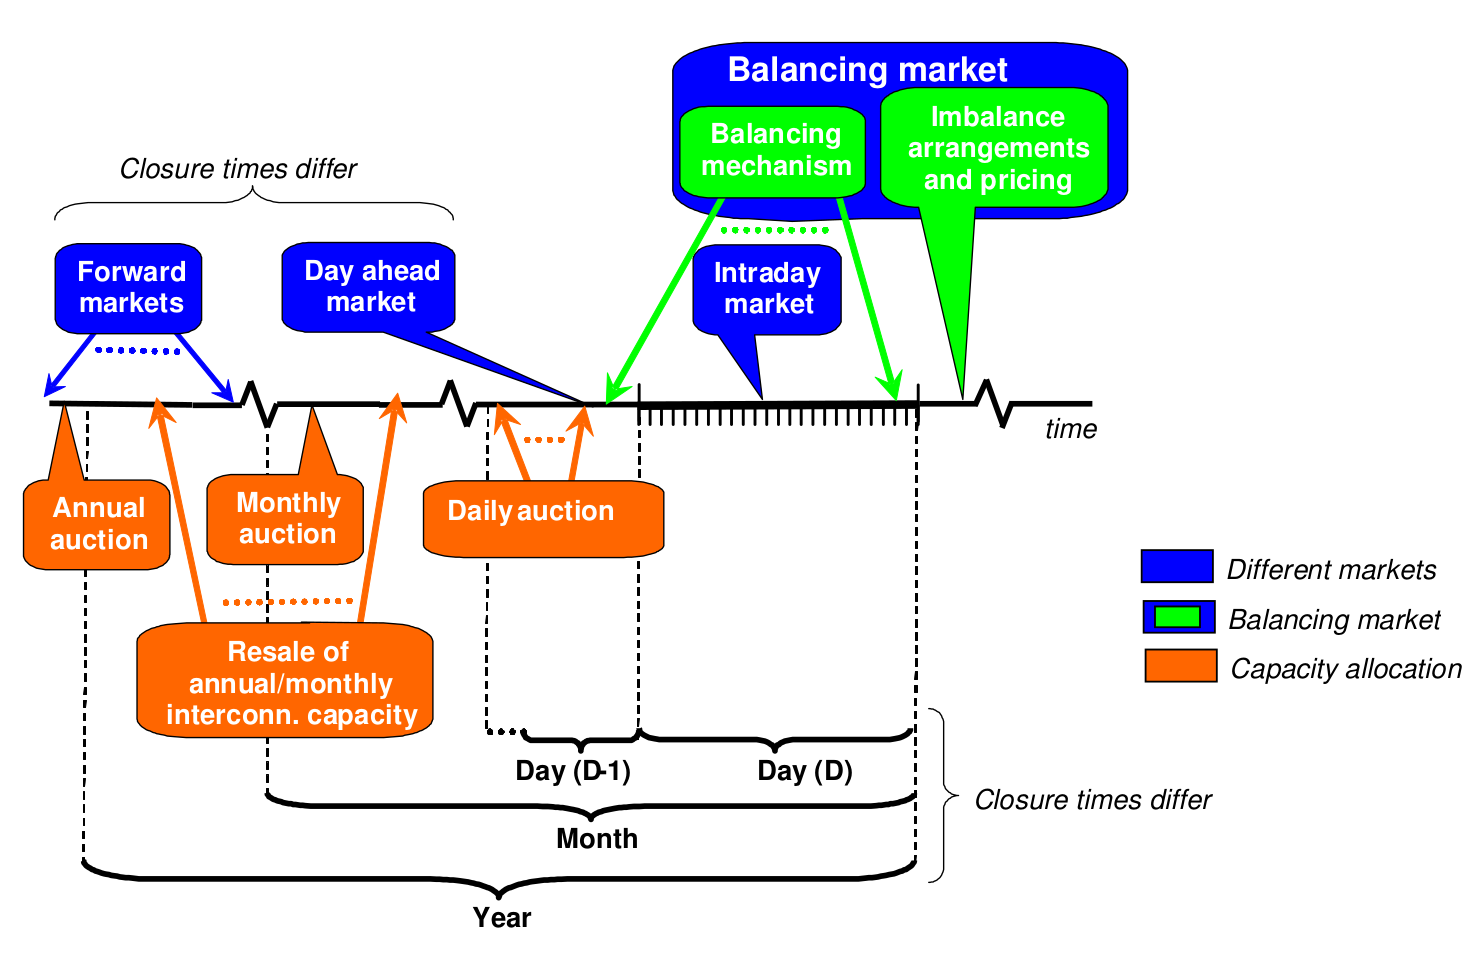
\includegraphics[width=0.95\linewidth]{./fig/electricity_markets.png}
\caption[Electricity Market Design]{Interaction between electricity markets in relation to capacity allocation \label{fig-electricity-markets}}
\end{figure}
\subsection{Electricity Market Theory:}
\label{sec:org57e3836}
\subsubsection{Balancing Market \label{sec-balancing-market}}
\label{sec:org792e1ec}
The balancing market is a tool to balance frequency deviations in the power
grid. It offers auctions for primary control reserve, secondary control reserve
as well as tertiary control reserve (minute reserve), which primarily differ in
the required ramp-up times of the participants. As depicted in Figure
\ref{fig-electricity-markets}, the balancing market can be seen as the last link
in a chain of electricity markets \cite{veen16_elect_balan_market}. In this study,
we will look at the German Control Reserve Market (GCRM), one of the largest
frequency regulation markets in the world. However, the presented concepts can
be easily transferred to other balancing markets in unbundled energy systems,
since the market design is similar
\cite{brandt17_evaluat_busin_model_vehic_grid_integ}. Transmission Systems
Operators (TSO) procure their required control reserve via tender auctions at
the GCRM. The market conducts daily auctions for the three types of control
reserve. This thesis focuses on the secondary operating reserve auction, in
which participants must be able to supply or absorb a minimum of 1MW of power
over a 4-hour interval with a reaction time of 30 seconds.\footnote{See \url{https://regelleistung.net}, accessed on 15\textsuperscript{th} February
2019, for further information on the market design and historical data.} Since EV
batteries can absorb energy almost instantly, when they are connected to a
charging station, they are suitable to provide such balancing services.
Operating reserve providers have to be qualified by the TSO to participate in
the market and are able to reliably provide the committed capacity. Although EV
fleets are currently not qualified by the GCRM to be used as operating reserve,
they could theoretically handle the minimum capacity requirements. Around 220
EVs would need to simultaneously charge at standard 4.6kW charging stations to
provide 1MW of downward regulating capacity.

Up until 28\textsuperscript{th} July 2018, auctions were held weekly, with two different
segments each week (peak hours/non-peak hours). Afterwards, the auction
mechanism changed to \emph{daily} auctions of six four-hour segments of positive and
negative control reserve.\footnote{\url{https://www.bundesnetzagentur.de/SharedDocs/Pressemitteilungen/DE/2017/28062017\_Regelenergie.html},
accessed 18\textsuperscript{th} February, 2019} Shorter auction cycles facilitate the
integration of renewable energy generators into the secondary control reserve
market, as they are dependent on accurate (short-term) capacity forecasts.

Positive control reserve is energy that is supplied to the grid, when the grid
frequency falls below 50Hz. It can be provided by increasing the electricity
generation or by reducing the grid load (i.e., electricity consumption). On the
contrary, negative control reserve is required when the grid frequency rises
above 50Hz and can be provided by adding grid load or reducing electricity
generation. Since we do not consider V2G in this thesis, the EV fleets in our
model are only able provide \emph{negative control reserve}, which we will refer to
as \emph{control reserve} until the end of the thesis. Market participants submit
bids in the following form to the market: \((\Pb{}, \cp{}, \ep{})\), where \(\Pb{}\)
is the amount of electrical power that can be supplied on demand in kW, \(\cp{}\) is
the capacity price for keeping the power available in \(\text{\euro{}/MW}\) and
\(\ep{}\) is the energy price for delivered energy in \(\text{\euro{}/MWh}\). The TSO
determines the target quantity of energy to acquire per timeslot, it usually
acquires much higher regulation capacity to minimize risks and activates the
capacity on demand. The TSO accepts the bids based on the capacity price in a
merit order. Providers, whose bids were accepted, instantly get compensated for
the provided capacity: \(R^c = \cp{} \times \Pb{}\). At the time regulation
capacity is needed, usually a day to a week later, the TSO activates the
capacity according to a merit order of the ascending \emph{energy prices} \(\ep{}\).
Hence, providers are also compensated according to the actual energy \(\Eb{}\)
they supplied or consumed: \(R^e = \ep{} \times \Eb{}\). Since provider get paid
according to their submitted price \(\ep{}\), instead of a market clearing price,
this type of auction is called \emph{pay-as-bid} auction.
\subsubsection{Spot Market \label{sec-spot-market}}
\label{sec:orge3f52a7}
As mentioned in the previous chapter, the equilibrium of electricity supply and
demand is ensured through a sequence of interdependent wholesale markets (cited)
\cite{pape16_are_fundam_enoug}. Next to the balancing market at the end of the
sequence, mainly two different types of spot markets exist, the day-ahead
market and the intraday market. In this research, we consider the European Power
Exchange (EPEX Spot) as it is the largest electricity market in Europe, with a
total trading volume of approximately 567TWh in 2018\footnote{\url{https://www.epexspot.com/en/press-media/press/details/press/Traded\_volumes\_soar\_to\_an\_all-time\_high\_in\_2018},
accessed 19\textsuperscript{th} February, 2019\label{org2b6afd4}}, but most electronic
spot markets in western economies work with similar market mechanisms.

In Germany, the most important spot market is the day-ahead market with a
trading volume of over 234TWh in 2018\textsuperscript{\ref{org2b6afd4}}. Participants place asks and bids
for hourly contracts of the following day on the \emph{EPEX Spot Day-ahead Auction}
market until the market closes at 12pm on the day before delivery (see Figure
\ref{fig-electricity-markets}). The day-ahead market plays an essential role in
integrating volatile renewable energy sources (RES) into the power system
\cite{pape16_are_fundam_enoug}. Generators forecast the expected generation
capacity for the next day and sell those quantities on the market
\cite{karanfil17_role_contin_intrad_elect_market}. After the market closes, the
participants have the opportunity to trade the difference between the day-ahead
forecast and the more accurate intraday forecast on the intraday market
\cite{kiesel17_econom_analy_intrad_elect_prices}. In this way, RES generators can
cost effectively self-balance their portfolios, instead of relying on balancing
services provided by the TSO, which imposes high imbalance costs on participants
\cite{pape16_are_fundam_enoug}.

On the \emph{EPEX Spot Intraday Continuous} market, electricity products are traded
up until 5 minutes before physical delivery. Hourly contracts, as well as
15-minute and block contracts, can be traded. In contrast to the day-ahead
auction, the intraday market is a continuous order-driven market. Participants
can submit limit orders at any time during the trading window and equally change
or withdraw the order at any time before the order is accepted. Limit orders are
specified as price-quantity pairs: \((\Pi{}, \up{})\), where \(\Pi{}\) is the
traded amount of electrical power in kW and \(\up{}\) is the price for the delivered
energy unit (hour/quarter/block) in \(\text{\euro{}/MWh}\). When an order to buy
(bid) matches an order to sell (ask), the trade immediately gets executed. The
order book is visible to all participants, hence it is known which unmatched
orders exist at the time of interest. The intraday market has a trading volume
of 82TWh, which is considerably smaller than day-ahead market's volume. Despite
that, the intraday market plays a vital role to the stability of the grid. All
executed trades on the intraday market potentially reduce the activation of
control reserve through the TSO.

Purchasing electricity on the continuous intraday market is attractive for EV
fleets with uncertain mobility demand. Due to the intradays market's short time
before delivery, EV fleet operators can rely on highly accurate forecasts of
available battery capacity to charge, before submitting an order to buy. In this
way, they can reliably charge at a potentially lower price at the intraday
market than the standard tariff. In an integrated bidding strategy, EV fleet
operators can, similarly to RES generators, balance out forecast errors of
available battery capacity on the intraday market. Trades on the intraday market
can complement bids that have been committed to other markets earlier (e.g., to
the secondary operating reserve market).
\subsection{EV Fleet Control in the Smart Grid}
\label{sec:org438ba97}
The increasing penetration of EVs has a substantial effect on electricity
consumption patterns. During charging periods, power flows and grid losses
increase considerably and challenge the grid. Operators have to reinforce the
grid to ensure that transformers and substations do not overload
\cite{sioshansi12_impac_elect_tarif_plug_in,lopes11_integ_elect_vehic_elect_power_system}.
Loading multiple EVs in the same neighborhood, or worse, whole EV fleets at
once, stress the grid. In these cases, even brown- or blackouts can occur.
\cite{kim12_carbit}. Despite these challenges, it is possible to support the
physical reinforcement by adopting smart charging strategies. In smart charging,
EVs get charged when the grid is less congested to ensure grid stability. Smart
charging reduces peaks in electricity demand, called \emph{Peak Cutting}, and
complement the grid in times of low demand, called \emph{Valley Filling}. Smart
charging has been researched thoroughly in the IS literature, in the following
we will outline some of the most important contributions.


\textcite{valogianni14_effec_manag_elect_vehic_storag} found that using
intelligent agents to schedule EV charging substantially reshapes the energy
demand and reduces peak demand without violating individual household
preferences. Moreover, they showed that the proposed smart charging behavior
reduces average energy prices and thus benefit households economically. In
another study, \textcite{kara15_estim_benef_elect_vehic_smart} investigated the
effect of smart charging on public charging stations in California. Controlling
for arrival and departure times, the authors presented beneficial results for
the distribution system operator (DSO) and the owners of EVs. Their approach
resulted in a price reduction in energy bills and a peak load reduction. An
extension of the smart charging concept is Vehicle-to-Grid (V2G). When equipped
with V2G devices, EVs can discharge their batteries back into the grid. Existing
research has focused on this technology in respect to grid stabilization effects
and arbitrage possibilities. For instance,
\textcite{schill11_elect_vehic_imper_elect_market} showed that the usage of EVs
can decrease average consumer electricity prices. Excess EV battery capacity can
be used to charge in off-peak hours and discharge in peak hours, when the prices
are higher. These arbitrage possibilities reverse welfare effects of generators
and increase the overall welfare and consumer surplus.
\textcite{tomic07_using_fleet_elect_drive_vehic_grid_suppor} found that the
arbitrage opportunities are especially prominent when a high variability in
electricity prices on the target electricity market exists. The authors stated
that short intervals between the contract of sale and the physical delivery of
electricity increase arbitrage benefits. Consequently, ancillary service
markets, like frequency control and operating reserve markets, are attractive
for smart charging.

\textcite{peterson10_econom_using_plug_in_hybrid} investigated energy arbitrage
profitability with V2G in the light of battery depreciation effects in the US.
The results of their study indicate that large-scale use of EV batteries for
grid storage does not yield enough monetary benefits to incentivize EV owners to
participate in V2G activities. Considering battery depreciation cost, the
authors arrived at an annual profit of only 6\$ - 72\$ per EV.
\textcite{brandt17_evaluat_busin_model_vehic_grid_integ} evaluated a business
model for parking garage operators operating on the German frequency regulation
market. When taking infrastructure costs and battery depreciation costs into
account, they conclude that the proposed vehicle-grid integration is not
profitable. Even with idealized assumptions about EV adoption rates in Germany
and altered auction mechanisms, the authors arrived at negative profits.
\textcite{kahlen17_fleet} used EV fleets to offer balancing services to the grid.
Evaluating the impact of V2G in their model, the authors conclude that V2G would
only be profitable if reserve power prices were twice as high. Considering the
results from the studies mentioned above, our research does not include V2G,
since only marginal profits are expected.

In order to maximize profits, it is essential for market participants to develop
successful bidding strategies. Several authors have investigated bidding
strategies to jointly participate in multiple markets
\cite{mashhour11_biddin_strat_virtual_power_plant_2,he16_optim_biddin_strat_batter_storag}.
\textcite{mashhour11_biddin_strat_virtual_power_plant_2} used stationary battery
storage to participate in the spinning reserve market and the day-ahead market
at the same time. The authors developed a non-equilibrium model, which solves
the presented mixed-integer program with Genetic Programming (GP). Contrarily,
we use a model-free RL agent that learns an optimal policy (i.e., a trading
strategy) from actions it takes in the environment (i.e., bidding on electricity
markets). Using a model-free approach is especially beneficial for us, since
additional unknown variables and constraints (i.e., customer mobility demand)
complicate the formulation of a mathematical model.

\textcite{he16_optim_biddin_strat_batter_storag} conducted similar research to
\textcite{mashhour11_biddin_strat_virtual_power_plant_2}. The authors additionally
incorporated battery life cycle in their profit maximization model, which proved
to be a decisive factor. In contrast to the authors, we jointly participated in
the secondary operating reserve and spot market with the \emph{non-stationary}
storage of EV batteries. Because shared EVs have to satisfy mobility demand,
they have to be charged in any case, which allows us to safely exclude battery
depreciation from our model. Further, we chose the intraday market over the
day-ahead market, as it has the lowest reaction time among the spot markets, and
thus potentially offers higher profits
\cite{tomic07_using_fleet_elect_drive_vehic_grid_suppor}.

Previous studies often assume that car owners or households can directly trade
on electricity markets. In reality, this is not possible due to the minimum
capacity requirements of the markets, requirements that single EVs do not meet.
For example, the German Control Reserve Market (GCRM) has a minimum trading
capacity of 1MW to 5MW, depending on the specific market. In order to reach the
minimum capacity, over 200 EVs would need to be connected to the grid via a
standard 4.6kW charging station at the same time. \textcite{ketter13_power_tac}
introduced the notion of electricity brokers, aggregators that act on behalf of
a group of individuals or households to participate in electricity markets.
\textcite{brandt17_evaluat_busin_model_vehic_grid_integ} and
\textcite{kahlen14_balan_with_elect_vehic} successfully showed that electricity
brokers can overcome the capacity issues by aggregating EV batteries. In
addition to electricity brokers, we apply the concept of Virtual Power Plants
(VPPs). VPPs are flexible portfolios of distributed energy resources, which are
presented with a single load profile to the system operator, making them
eligible for market participation and ancillary service provisioning
\cite{pudjianto07_virtual_power_plant_system_integ}. Hence, VPPs allow providing
regulation capacity to the market without knowing which exact sources provide
the promised capacity until the delivery time \cite{kahlen17_fleet}. This concept
is specially useful when dealing with EV fleets: VPPs enable carsharing
providers to issue bids and asks based on an estimate of available fleet
capacity, without knowing beforehand which exact EVs will provide the capacity
at the time of delivery. Based on the battery charge and the availability of
EVs, an intelligent agent decides in real-time which vehicles provide the
capacity.

Centrally managed EV fleets make it possible for carsharing providers to use the
presented concepts as a viable business extension. Free float carsharing is a
popular concept that allows cars to be picked up and parked everywhere, and the
customers are billed is by the minute. Free float carsharing offers flexibility
to its users, saves resources, and reduces carbon emissions
\cite{firnkorn15_free_float_elect_carsh_fleet_smart_cities}. Most previous studies
concerned with the usage of EVs for electricity trading, assumed that trips are
fixed and known in advance, e.g., in
\textcite{tomic07_using_fleet_elect_drive_vehic_grid_suppor}. The free float
concept adds uncertainty and nondeterministic behavior, which make predictions
about future rentals a complex issue.

\textcite{kahlen17_fleet} showed that it is possible to use free float carsharing
fleets as VPPs to profitably offer balancing services to the grid. In their
study, the authors compared cases from three different cities across Europe and
the US. They used an event-based simulation, bootstrapped with real-world
carsharing and secondary operating reserve market data from the respective
cities. A central dilemma within their research was to decide whether an EV
should be committed to a VPP or free for rent. Since rental profits are
considerably higher than profits from electricity trading, it is crucial not to
allocate an EV to a VPP when it could have been rented out otherwise. To deal
with the asymmetric payoff, \citeauthor{kahlen17_fleet} used stratified sampling
in their classifier. This method gives rental misclassifications higher weights,
reducing the likelihood of EVs to participate in VPP activities. The authors
used a Random Forest regression model to predict the available balancing
capacity on an aggregated fleet level. Only at the delivery time, the agent
decides which individual EVs provide the regulation capacity. This heuristic is
based on the likelihood that the vehicle is rented out and on its expected
rental benefits.

In a similar study, the authors showed that carsharing companies can participate
in day-ahead markets for arbitrage purposes
\cite{kahlen18_elect_vehic_virtual_power_plant_dilem}. In the paper, the authors
used a sinusoidal time-series model to predict the available trading capacity.
Another central problem for carsharing providers is that committed trades, which
can not be fulfilled, result in substantial penalties from the system operator
or electricity exchange. In other words, fleet operators have to avoid buying
any amount of electricity, which they can't be sure to charge with available EVs
at the delivery time. To address this issue, the authors developed a mean
asymmetric weighted (MAW) objective function. They used it for their time-series
based prediction model, to penalize committing an EV to VPP when it would have
been rented out otherwise. Because of the two issues mentioned above,
\textcite{kahlen18_elect_vehic_virtual_power_plant_dilem} could only make very
conservative estimations and commitments of overall available trading capacity,
resulting in a high amount of foregone profits. This effect is especially
prominent when participating in the secondary operating reserve market, since
commitments have to be made one week in advance when mobility demands are still
uncertain. \textcite{kahlen17_fleet} stated that in 42\% to 80\% of the cases, EVs
are \emph{not} committed to a VPP when it would have been profitable to do so.

This thesis proposes a solution in which the EV fleet participates in the
balancing market and intraday market simultaneously. With this approach, we
align the potentially higher profits on the balancing markets, with more
accurate capacity predictions for intraday markets
\cite{tomic07_using_fleet_elect_drive_vehic_grid_suppor}. This research followed
\textcite{kahlen17_fleet}, who proposed to work on a combination of multiple
markets in the future.

\subsection{Reinforcement Learning Controlled EV Charging}
\label{sec:org3a595e6}

Previous research shows that intelligent agents equipped with Reinforcement
Learning (RL) methods can successfully take action in the smart grid. The
following chapter outlines different research approaches of RL in the domain of
smart grids. For a more thorough description, mathematical formulations and
common issues, of RL refer to Chapter \ref{sec-reinforcement-learning}.

\textcite{reddy11_learn_behav_multip_auton_agent,reddy11_strat} used autonomous
broker agents to buy and sell electricity from DER on a proposed \emph{Tariff
Market}. The agents use Markov Decision Processes (MDPs) and RL to learn pricing
strategies to profitably participate in the Tariff Market. To control for a
large number of possible states in the domain, the authors used \emph{Q-Learning}
with derived state space features. Based on descriptive statistics, they defined
derived price and market participant features. By engaging with its environment,
the agent learns an optional sequence of actions (policy) based on the state of
the agent. \textcite{peters13_reinf_learn_approac_to_auton} built on that work and
further enhanced the method by using function approximation. Function
approximation allows to efficiently learn strategies over large state spaces, by
deriving a function that describes the states instead of defining discrete
states. By using this technique, the agent can adapt to arbitrary economic
signals from its environment, resulting in better performance than previous
approaches. Moreover, the authors applied feature selection and regularization
methods to explore the agent's adaption to the environment. These methods are
particularly beneficial in smart markets because market design, structures, and
conditions might change in the future. Hence, intelligent agents should be able
to adapt to it \cite{peters13_reinf_learn_approac_to_auton}.

\textcite{vandael15_reinf_learn_heuris_ev_fleet} facilitated learned EV fleet
charging behavior to optimally purchase electricity on the day-ahead market.
Similarly to \textcite{kahlen18_elect_vehic_virtual_power_plant_dilem}, the
problem is framed from the viewpoint of an aggregator that tries to define a
cost-effective day-ahead charging plan in the absence of knowing EV charging
parameters, such as departure time. A crucial point of the study is weighting
low charging prices against costs that have to be paid when an excessive or
insufficient  amount of electricity is bought from the market (imbalance costs).
Contrarily, \textcite{kahlen18_elect_vehic_virtual_power_plant_dilem} did not
consider imbalance cost in their model and avoid them by sacrificing customer
mobility in order to balance the market (i.e., not showing the EV available for
rent, when it is providing balancing capacity).
\textcite{vandael15_reinf_learn_heuris_ev_fleet} used a \emph{fitted Q Iteration} to
control for continuous variables in their state and action space. In order to
achieve fast convergence, they additionally optimized the \emph{temperature step}
parameter of the Boltzmann exploration probability.

\textcite{dusparic13_multi} proposed a multi-agent approach for residential demand
response. The authors investigated a setting in which 9  EVs were connected to
the same transformer. The RL agents learned to charge at minimal costs, without
overloading the transformer. \textcite{dusparic13_multi} utilized \emph{W-Learning} to
simultaneously learn multiple policies (i.e., objectives such as ensuring
minimum battery charged or ensuring charging at low costs).
\textcite{taylor14_accel_learn_trans_learn} extended this research by employing
Transfer Learning and \emph{Distributed W-Learning} to achieve communication between
the learning processes of the agents in a multi-objective, multi-agent setting.
\textcite{dauer13_market_based_ev_charg_coord} proposed a market-based EV fleet
charging solution. The authors introduced a double-auction call market where
agents trade the available transformer capacity, complying with the minimum
required State of Charge (SoC). The participating EV agents autonomously learn
their bidding strategy with standard \emph{Q-Learning} and discrete state and action
spaces.

\textcite{di13_elect_vehic} presented a multi-agent solution to minimize charging
costs of EVs, a solution that requires neither prior knowledge of electricity
prices nor future price predictions. Similar to
\textcite{dauer13_market_based_ev_charg_coord}, the authors employed standard
\emph{Q-Learning} and the \(\epsilon\)-greedy approach for action selection.
\textcite{vaya14_optim} also proposed a multi-agent approach, in which the
individual EVs are agents that actively place bids in the spot market. Again,
the agents use \emph{Q-Learning}, with an \(\epsilon\)-greedy policy to learn their
optimal bidding strategy. The latter relies on the agents willingness-to-pay
which depends on the urgency to charge. State variables, such as SoC, time of
departure and price development on the market, determine the urgency to charge.
The authors compared this approach with a centralized aggregator-based approach
that they developed in another paper \cite{vaya15_optim_biddin_strat_plug_in}.
Compared to the centralized approach, in which the aggregator manages charging
and places bids for the whole fleet, the multi-agent approach causes slightly
higher costs but solves scalability and privacy problems.

\textcite{shi11_real} consider a V2G control problem, while assuming real-time
pricing. The authors proposed an online learning algorithm which they modeled as
a discrete-time MDP and solved through \emph{Q-Learning}. The algorithm controls the
V2G actions of the EV and can react to real-time price signals of the market. In
this single-agent approach, the action space compromises only charging,
discharging and regulation actions. The limited action spaces makes it
relatively easy to learn an optimal policy.
\textcite{chis16_reinf_learn_based_plug_in} looked at reducing the costs of
charging for a single EV using known day-ahead prices and predicted next-day
prices. A Bayesian ANN was employed for prediction and \emph{fitted Q-Learning} was
used to learn daily charging levels. In their research, the authors used
function approximation and batch reinforcement learning, an offline, model-free
learning method. \textcite{ko18_mobil_aware_vehic_to_grid} proposed a centralized
controller for managing V2G activities in multiple microgrids. The proposed
method considers mobility and electricity demands of microgrids, as well as SoC
of the EVs. The authors formulated a MDP with discrete state and action spaces
and use standard \emph{Q-Learning} with \(\epsilon\)-greedy policy to derive an optimal
charging policy. The approach takes microgrid autonomy and electricity prices
into special consideration.

It should be noted that advanced RL methods and techniques are not the only
solutions for problems in the smart grid, often basic algorithms and heuristics
provide satisfactory results \cite{vazquez-canteli19_reinf_learn_deman_respon}.
Despite that, our paper considers RL as an optimal fit for the design of our
proposed intelligent agent. Given the ability to learn user behavior (e.g.,
mobility demand) and the flexibility to adapt to the environment (e.g.,
electricity prices), RL methods are a promising way of solving complex
challenges in smart grids.

\clearpage
\subsection{Reinforcement Learning Theory \label{sec-reinforcement-learning}}
\label{sec:orgcb6cdb7}
The following chapter will give an overview of the most important Reinforcement
Learning (RL) concepts and will introduce the corresponding mathematical
formulations. If not noted otherwise, the notation, equations, and insights are
adopted from \cite{sutton18_reinf}, the de-facto reference book of RL research.

RL is an agent-based machine learning algorithm in which the agent learns to
perform an optimal set of actions through interaction with its environment. The
agents objective is to maximize the rewards it receives based on the actions it
takes. Immediate rewards have to be weighted against long-term cumulative
returns that also on its future actions. The RL problem is formalized as Markov
Decision Processes (MDPs) which will be introduced in Chapter \ref{sec-mdp}. A
critical task of RL agents is to continuously estimate the value of the
environments state. Values indicate the long-term desirability of a state, that
is the total amount of reward the agent can expect to accumulate over the
future, following a learned set of actions, called the policy. Policies and
values are covered in Chapter \ref{sec-policies}, whereas the core mathematical
foundations for evaluating policies and updating value functions are introduced
in Chapter \ref{sec-bellman}. When the model of the environment is fully known,
the learning problem is reduced to a planning problem (Chapter \ref{sec-dp}) in
which optimal policies can be computed with iterative approaches. Model-free RL
approaches can be applied when rewards and state transitions are unknown, and
the agent's behavior has to be learned from experience (Chapter
\ref{sec-td-learning}). The last two chapter cover methods that solve the RL
problem more efficiently, tackle new challenges and are widely used in practice
and research.

\subsubsection{Markov Decision Processes \label{sec-mdp}}
\label{sec:org156af44}
Markov Decision Processes (MDPs) are a classical formulation of sequential
decision making and an idealized mathematical formulation of the RL problem. MDPs
allow to derive exact theoretical statements about the learning problem and
possible solutions. Figure
\ref{agent-environment-interaction} depicts the \emph{agent-environment interaction}.
\begin{figure}[htbp]
\centering
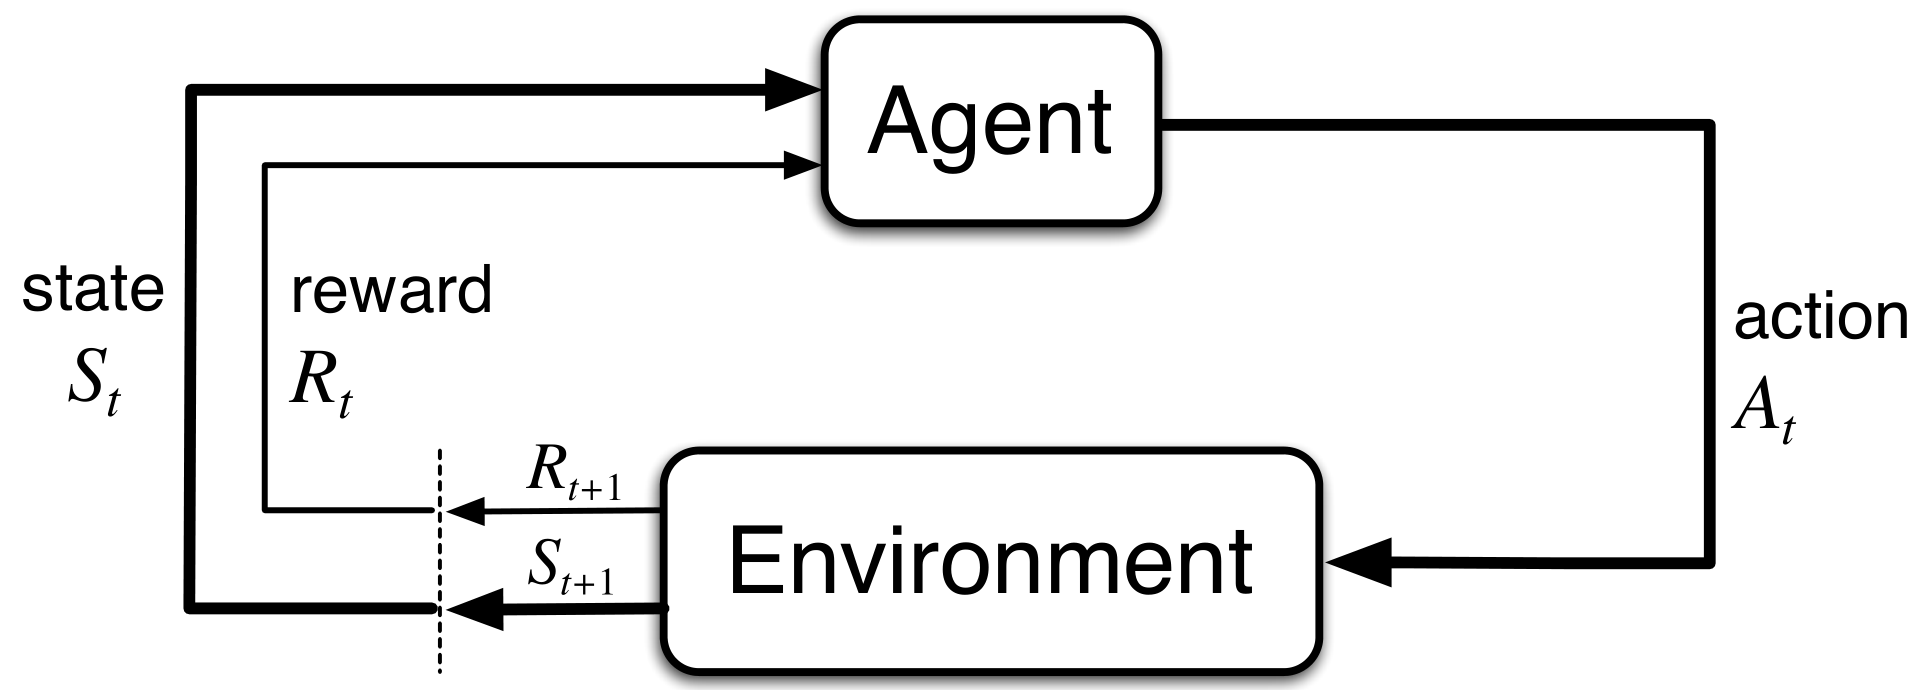
\includegraphics[width=0.95\linewidth]{./fig/mdp_interaction.png}
\caption[Markov Decision Process]{The agent-environment interaction in a Markov decision process \cite{sutton18_reinf} \protect\footnotemark \label{agent-environment-interaction}}
\end{figure}
\footnotetext{\textbf{Figure 3.1} from "Reinforcement Learning: An Introduction" by Richard S. Sutton and Andew G. Barto is licencsed under CC BY-NC-ND 2.0 (https://creativecommons.org/licenses/by-nc-nd/2.0/)}

In RL the agent and the environment continuously interact with each other. The
agent takes actions that influence the environment, which in return presents
rewards to the agent. The agent's goal is to maximize rewards over time, trough
an optimal choice of actions. In each discrete timestep \(t\!=\!0,1,2,...,T\) the
RL agent interacts with the environment, which is perceived by the agent as a
representation, called \emph{state}, \(S_t \in \S\). Based on the state, the agents
selects an \emph{action}, \(A_t\in\A\), and receives a numerical \emph{reward} signal,
\(R_{t+1}\in\R\subset\Re\), in the next timestep. Actions influence immediate
rewards and successive states, and consequently also influence future rewards.
The agent has to continuously make a trade-off between immediate rewards and
delayed rewards to achieve its long-term goal.

The \emph{dynamics} of a MDP are defined by the probability that a state \(s'\in \S\)
and a reward \(r\in\R\) occurs, given the preceding state \(s\in\S\) and action
\(a\in\A\). In \emph{finite} MDPs, the random variables \(\R_t\) and \(S_t\) have
well-defined probability density functions (PDF), which are solely dependent on
the previous state and action. Consequently, it is possible to define (\(\defeq\))
the \emph{dynamics} of the MDP as follows:
\begin{equation}
    p(s',r|s,a) \defeq \Pr{S_t=s',R_t=r|S_{t-1}=s,A_t=a},
\end{equation}
for all \(s',s\!\in\!\S\), \(r\!\in\!\R\) and \(a\!\in\!\A\). Note that each possible
value of the state \(\S_t\) depends only on the immediately preceding state
\(\S_{t-1}\). When a state includes all information of \emph{all} previous states, the
state possesses the so-called \emph{Markov property}. If not noted otherwise, the
Markov property is assumed throughout the whole chapter. The dynamics function
allows computing the \emph{state-transition probabilities}, another important
characteristic of an MDP, as follows:
\begin{equation}
    p(s'|s,a) \defeq \Pr{S_t\!=\!s'|S_{t-1}\!=\!s,A_t\!=\!a} = \sum_{r\in\R}{p(s', r|s, a)},
\end{equation}
for \(s',s\!\in\!\S\), \(r\!\in\!\R\) and \(a\!\in\!\A\).

The use of a \emph{reward signal} \(R_t\) to formalize the agent's goal is a unique
characteristic of RL. Each timestep the agent receives the rewards as a scalar
value \(\R_t\in\Re\). The sole purpose of the RL agent is to maximize the
long-term cumulative reward (as opposed to the immediate reward). The long-term
cumulative reward can also be expressed as the \emph{expected return} \(G_t\):
\begin{equation} \label{eq-expected-return}
\begin{split}
    G_t &\defeq R_{t+1} + \gamma R_{t+2} + \gamma R_{t+3} + \cdots \\
    &= \sum_{k=0}^{\infty}{\gamma^k R_{t+k+1}} \\
    &= R_{t+1} + \gamma G_{t+1},
\end{split}
\end{equation}
where \(\gamma\), \(0\leq\gamma\leq 1\), is the \emph{discount rate} parameter. The
discount rate determines how "myopic" the agent is. If \(\gamma\) approaches 0,
the agent is more concerned with maximizing immediate rewards. On the contrary,
when \(\gamma\!=\! 1\), the agent takes future rewards strongly into account, the
agent is "farsighted".

\subsubsection{Policies and Value Functions \label{sec-policies}}
\label{sec:org3d8a795}
An essential task of almost every RL agent is estimating \emph{value functions}.
These functions describe how "good" it is to be in a given state, or how "good"
it is to perform an action in a given state. More formally, they take a state
\(s\) or a state-action pair \(s,a\) as input and give the expected return \(G_t\) as
output. The expected return is dependent on the actions the agent will take in
the future. Consequently, value functions are formulated with respect to a
\emph{policy} \(\pi\). A policy is a mapping of states to actions; it describes the
probability that an agent performs a certain action, based on the current state.
More formally, the policy is defined as
\(\pi(a|s)\defeq\Pr{A_t\!=\!a|S_t\!=\!s}\), a PDF of all \(a\!\in\!\A\) for each
\(s\!\in\!\S\). RL approaches mainly differ in how the policy is updated, based on
the agent's interaction with the environment.

In RL, value functions of states and value functions of state-action pairs are
used. The \emph{state-value function of policy} \(\pi\) is denoted as \(\vpi(s)\) and is
defined as the expected return when starting in \(s\) and following policy \(\pi\):
\begin{equation}
    \vpi(s) \defeq \EE{\pi}{G_t|S_t\!=\!s}, \text{ for all } s\in\S
\end{equation}
The \emph{action-value function of policy} \(\pi\) is denoted as \(\qpi(s,a)\) and is
defined as the expected return when starting in \(s\), taking action \(a\) and
following policy \(\pi\) afterwards:
\begin{equation}
    \qpi(s,a) \defeq \EE{\pi}{G_t|S_t\!=\!s, A_t\!=\!a}, \text{ for all } a\in\A, s\in\S
\end{equation}
The \emph{optimal policy} \(\pi_*\) has a greater (or equal) expected return than all
other policies.  The \emph{optimal} state-value function and \emph{optimal} action-value
function are defined as follows:
\begin{equation}
    \vstar(s) \defeq \max_{\pi} \vpi(s), \text{ for all } s\in\S
\end{equation}
\begin{equation}
    \qstar(s,a) \defeq \max_{\pi} \qpi(s,a), \text{ for all } s\in\S, a\in\A
\end{equation}
The \emph{optimal} action-value function describes the expected return when taking
action \(a\) in state \(s\) following the optimal policy \(\pi_*\) afterwards.
Estimating \(\qstar\) to obtain an optimal policy is a substantial part of RL and
has been known as \emph{Q-learning} \cite{watkins92_q_learn}, which is described in
Chapter \ref{sec-td-learning}.

\subsubsection{Bellman Equations \label{sec-bellman}}
\label{sec:orgfdac7e4}
A central characteristic of value functions is the recursive relationship
between the values. Similar to Equation (\ref{eq-expected-return}), current values
are related to expected values of successive states. This relationship is
heavily used in RL and has been formulated as \emph{Bellman equations}
\cite{bellman57_dynam_progr}. The Bellman equation for \(\vpi(s)\) is defined as
follows:
\begin{equation} \label{eq-bellman}
\begin{split}
    \vpi(s) &\defeq \EE{\pi}{G_t|S_t=s} \\
    &= \EE{\pi}{R_{t+1}+\gamma G_{t+1}|S_t\!=\!s} \\
    &= \sum_{a}{\pi(a|s)}\sum_{s',r}{p(s',r|s,a)}\bigg[r+\gamma\vpi(s')\bigg],
\end{split}
\end{equation}
where \(a\!\in\!\A\), \(s,s'\!\in\!\S\), \(r\!\in\!\R\).
In other words, the value of a state equals the immediate reward plus the
expected value of all possible successor states, weighted by their probability
of occurring. \(\vpi(s)\) is the only solution to its Bellman equation. The
Bellman equation of the optimal value function \(v_*\) is called the \emph{Bellman
optimality equation}:
\begin{equation} \label{eq-bellman-optimality}
\begin{split}
    \vstar(s) &= \max_{a\in\A(s)}q_{\pi_*}(s,a) \\
    &= \max_{a}\EE{\pi_*}{R_{t+1}+\gamma G_{t+1}|S_t\!=\!s, A_t\!=a} \\
    &= \max_{a}\EE{\pi_*}{R_{t+1}+\gamma \vstar(S_{t+1})|S_t\!=\!s, A_t\!=a} \\
    &= \max_{a}\sum_{s',r}{p(s',r|s,a)}\bigg[r+\gamma\vstar(s')\bigg]
\end{split}
\end{equation}
where \(a\!\in\!\A\), \(s,s'\!\in\!\S\), \(r\!\in\!\R\). In other words, the value of
a state under an optimal policy equals the expected return for the best action
from that state. Note that the Bellman optimality equation does not refer to a
specific policy, it has a unique solution independent from one. It can be seen
as an equation system, which can be solved when the dynamics of the environment
\(p\) are known. Similar Bellman equations to Equations (\ref{eq-bellman}) and
(\ref{eq-bellman-optimality}) can also be formed for \(\qpi(s,a)\) and
\(\qstar(s,a)\). Bellman equations form the basis for computing and approximating
value functions and were an important milestone in RL history. Most RL methods
are \emph{approximately} solving the Bellman optimality equation, by using
experienced state transitions instead of expected transition probabilities. The
most common methods will be explored in the following chapters.

\subsubsection{Dynamic Programming  \label{sec-dp}}
\label{sec:org7c67728}
\emph{Dynamic Programming} (DP) is a method to compute optimal policies, the primary
goal of every RL method. DP makes use of value functions to facilitate the
search for good policies. Once an optimal value function, (i.e., one that
satisfies the Bellman optimality equation) is found, optimal policies can be
easily obtained. Despite the limited utility of DP in real-world settings, it
provides the theoretical foundation for all other RL methods. In fact, all of
the RL methods try to achieve the same goal, but without the assumption of a
perfect model of the environment and less computational effort. Because DP assumes
full knowledge of the environment, it is known as \emph{planning}, in which optimal
solutions are \emph{computed}. In \emph{control} problems (Chapter \ref{sec-td-learning}),
optimal solutions are \emph{learned} from an unknown environment.

The two most popular DP algorithms that compute optimal policies are called
\emph{policy iteration} and \emph{value iteration}. These methods perform "sweeps" through
the whole state set and update the estimated value of each state via an
\emph{expected update} operation. In policy iteration, a value function for a given
policy \(\vpi\) needs to be computed first, a step called \emph{policy evaluation}. A
sequence of approximated value functions \(\{v_k\}\) are updated using the Bellman
equation for \(\vpi\) (Eq. \ref{eq-bellman}) until convergence to \(\vpi\) is
achieved. After computing the value function for a given policy, it is possible
to modify the policy and see if the value \(\vpi(s)\) for a given state increases
(\emph{policy improvement}). A way of doing this, is evaluating the action-value
function \(\qpi(s,a)\) by \emph{greedily} taking the best short-term action \(a\!\in\!A\)
at a given timestep. Alternating between these two steps monotonically improves
the policies and the value functions until they converge to the optimum. This
algorithm is called \emph{policy iteration}:
\begin{equation}
    \pi_0 \xrightarrow{\text{ E }} v_{\pi_0} \xrightarrow{\text{ I }}
    \pi_1 \xrightarrow{\text{ E }} v_{\pi_1} \xrightarrow{\text{ I }}
    \pi_2 \xrightarrow{\text{ E }} \hdots \xrightarrow{\text{ I }}
    \pi_* \xrightarrow{\text{ E }} \vstar,
\end{equation}
where \(\xrightarrow{\text{ E }}\) denotes a policy evaluation step,
\(\xrightarrow{\text{ I }}\) denotes a policy improvement step. \(\pi_*\) and
\(\vstar\) are the optimal policy and optimal value function, respectively. Note
that in each iteration of the policy iteration algorithm, a policy evaluation
has to be performed, which requires multiple sweeps through the state space. In
\emph{value iteration}, the policy evaluation step is stopped after one sweep. In
this case, the two previous steps can be combined into one single update step:
\begin{equation}
\begin{split}
    v_{k+1}(s) &\defeq \max_a \EE{}{R_{t+1}+\gamma \vstar(S_{t+1})|S_t\!=\!s, A_t\!=a} \\
    &= \max_{a}\sum_{s',r}{p(s',r|s,a)}\bigg[r+\gamma v_k(s')\bigg],
\end{split}
\end{equation}
where \(a\!\in\!\A\), \(s,s'\!\in\!\S\), \(r\!\in\!\R\). It can be shown, that for any
given \(v_0\), the sequence \({v_k}\) converges to the optimal value function
\({\vstar}\). In value iteration, the Bellman optimality equation
(\ref{eq-bellman-optimality}) is simply turned into an update rule. Both of the
algorithms can be effectively used to compute optimal values and value function
in finite MDPs with a perfect model of the environment.

\subsubsection{Temporal-Difference Learning \label{sec-td-learning}}
\label{sec:org61d04d7}
The previous chapter dealt with solving a \emph{planning} problem, that is computing
an optimal solution (i.e., an optimal policy \(\pi_*\)) of an MDP when a perfect
model of the environment is known. In the following chapters, we will look at
\emph{model-free} prediction and \emph{model-free} control. As opposed to planning,
model-free methods learn from experience and require no prior knowledge of the
environment. Remarkably, these methods can still achieve optimal behavior.

The \emph{TD prediction problem} is concerned with estimating state-values \(\vpi\)
using past experiences of following a given policy \(\pi\). TD methods update an
estimate \(V\) of \(\vpi\) in every timestep. At time \(t\!+\!1\) they immediately
perform an update operation on \(V(S_t)\). Because of the step-by-step nature of
TD learning, it is categorized as \emph{online learning}. Also note that TD methods
perform update operations on value estimates based on other learned estimates, a
procedure called \emph{bootstrapping}. In simple TD prediction, the
value estimates \(V\) are updated as follows:
\begin{equation} \label{eq-td-prediction}
    V(S_t) \leftarrow V(S_t) + \alpha\big[R_{t+1}+\gamma V(S_{t+1}) - V(S_t)\big],
\end{equation}
where \(\alpha\) is a constant \emph{step-size} parameter and \(\gamma\) is the
\emph{discount rate}. Here, the update of the state-value is performed using the
observed reward \(R_{t+1}\) and the estimated value \(V(S_{t+1})\).

When a model is not available, it is useful to estimate \emph{action-values}, instead
of \emph{state-values}. If the environment is completely known, it is possible for
the agent to look one step ahead and select the best action. Without that
knowledge, the value of each action in a given state needs to be estimated. The
latter constitutes a problem, since not every \emph{state-action} pair will be
visited when the agent follows a deterministic policy. A deterministic policy
\(\pi(a|s)\) returns exactly one action given the current state, hence the agent
will only observe returns for one of the actions. In order to evaluate the value
function for all \emph{state-action} pairs \(\qpi\), continuous \emph{exploration} needs to
be ensured. In other words, the agent has to explore state-action pairs which
are seemingly disadvantageous given the current policy. This dilemma is also
known as the \emph{exploration-exploitation} trade-off. One way to achieve exploration
is using \emph{stochastic} policies for the action selection. Stochastic policies
have a non-zero probability of selecting each action in each state. A typical
stochastic policy is the \emph{\(\epsilon\)-greedy policy}, which selects the action with
the highest estimated value, except for a probability \(\epsilon\), it selects an
action at random.
\begin{figure}[htbp]
\centering
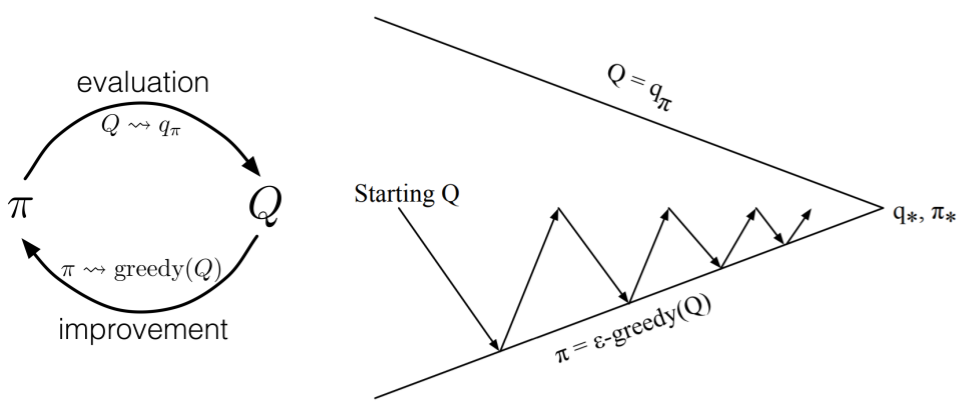
\includegraphics[width=0.95\linewidth]{./fig/on-policy.png}
\caption[On-policy control with Sarsa]{On-policy control with Sarsa \cite{sutton18_reinf}. \protect\footnotemark \label{fig-sarsa}}
\end{figure}
\footnotetext{The in-text figure of \textbf{Chapter 5.3} from "Reinforcement Learning: An Introduction" by Richard S. Sutton and Andew G. Barto is licencsed under CC BY-NC-ND 2.0 (https://creativecommons.org/licenses/by-nc-nd/2.0/)}

There are two approaches to make use of stochastic policies to ensure all
actions are chosen infinitely often. On-policy methods improve the (stochastic)
decision policy, by continually estimating \(\qpi\) in regard to \(\pi\), while
simultaneously driving \(\pi\) towards \(\qpi\), e.g., with a \(\epsilon\)-greedy action
selection. Figure \ref{fig-sarsa} depicts this learning process. Off-policy
methods improve the deterministic decision policy, by using a second stochastic
policy to generate behavior. The first policy is becoming the optimal policy by
evaluating the exploratory behavior of the second policy. Off-policy approaches
are considered more powerful than on-policy approaches and have a variety of
additional use cases. On the other side, they often have a higher variance and
take more time to converge to an optimum.

A popular on-policy TD control method is Sarsa, developed by
\textcite{rummery94_q}. In the prediction step, the action-value function
\(\qpi(s,a)\) of all actions and states has to be estimated for the current
policy \(\pi\). The estimation can be done similar to TD prediction of state
values (Eq. \ref{eq-td-prediction}). Instead of considering state transitions,
state-action transitions are considered in this case. The update rule is
constructed as follows:
\begin{equation}
    Q(S_t, A_t) \leftarrow Q(S_t,A_t) + \alpha\big[R_{t+1}+\gamma Q(S_{t+1},A_{t+1}) - Q(S_t, A_t)\big]
\end{equation}
After every transition from a state \(S_t\), an update operation using the events
\((S_t, A_t, R_{t+1}, S_{t+1}, A_{t+1})\) is performed. This quintuple also
constituted the name Sarsa. The on-policy control step of the algorithm is
straightforward, and uses a \(\epsilon\)-greedy policy improvement, as described in
the previous paragraph. It has been shown that Sarsa converges to the optimal
policy \(\pi_*\) under the assumption of infinite visits to all state-action
pairs.

A breakthrough in RL has been achieved when \textcite{watkins92_q_learn} developed
the \emph{off-policy} TD control algorithm, called Q-learning. The update rule is
defined as follows:
\begin{equation}
    Q(S_t, A_t) \leftarrow Q(S_t,A_t) + \alpha\big[R_{t+1}+\gamma\max_a Q(S_{t+1},a) - Q(S_t, A_t)\big]
\end{equation}
Here, the estimated action-values \(Q\) are updated towards the highest estimated
action-value of the next time step. In this way, \(Q\) directly approximates the
optimal action-value function \(q_*\), independently of the policy the agent
follows. Due to this simplification, Q-learning is a widely used model-free
method, and its convergence can be proved easily.


This chapter covered the most important RL methods. They work online, learn from
experience, and can be easily applied to real-world problems with low
computational effort. Moreover, the mathematical complexity of the presented
approaches is limited, and they can be easily implemented into computer
programs. Temporal-Difference learning is a \emph{tabular} method, in which Q-values
are stored and updated in a lookup table. If the state and action spaces are
continuous or the number of states and actions is very large, a table
representation is computational infeasible and the speed of convergence is
drastically reduced. In this case, a \emph{function approximator} can replace the
lookup table. The next chapter will briefly cover function approximation, as
well as other advancements in RL.
\subsubsection{Approximation Methods}
\label{sec:org670e7b4}
Up to this point, only tabular RL methods have been covered, which form the
theoretical foundation of RL in general. But in many real-world use cases, the
state space is enormous and it is improbable to find an optimal value function
with tabular methods. Not only is it a problem to store such a large table in
the memory, but also would it take an almost infinite amount of time to fill
every entry with meaningful results. Contrarily, \emph{function approximation} tries
to find a function that approximates the optimal value function as closely as
possible, with limited computational resources. The experience with a small
subset of visited states is generalized to approximate values of the whole state
set. Function approximation has been widely studied in supervised machine
learning: Gradient methods, as well as linear and non-linear models have shown
good results for RL.

The approximated value of a state \(s\) is denoted as the parameterized
functional form \(\hat v(s,\w)\!\approx\!\vpi(s)\), given a weight vector
\(\w\!\in\!\Re^d\). Function approximation methods are approximating \(\vpi\) by
learning (i.e., adjusting) the weight vector \(\w\) from the experience of following
the policy \(\pi\). By assumption, the dimensionality \(d\) of \(\w\) is much lower than
the number of states, which is the reason for the desired generalization effect:
Adjusting one weight affects the values of many states. However, optimizing
an estimate for one state negatively affects the accuracy of the estimates for
other states. This effect motivates the specification of a state distribution
\(\mu(s)\), which represents the importance of the prediction error for each state.
In on-policy prediction, \(\mu(s)\) is often selected to be proportion of time spend
in each state \(s\). The prediction error of a state is defined as the squared
difference between the predicted (i.e., approximated) value \(\hat v(s,\w)\) and
the true value \(\vpi(s)\). Consequently, the objective function of the supervised
learning problem can be defined as the \emph{Mean Squared Value Error} \(\MSVEm\),
which weights the prediction error with the state distribution \(\mu(s)\):
\begin{equation}
    \MSVEm(\w) \defeq \sum_{s\in\S}{\mu(s)\bigg[\vpi(s)-\hat v(s,\w)\bigg]^2}, \text{ where } \w\in\Re^d
\end{equation}
Minimizing \(\MSVEm\) in respect to \(\hat v\) will yield a value function, which
facilitates finding a better policy --- the primary goal of RL. Remember that \(\hat v\)
can take any form of a linear or non-linear function of the state \(s\).

In practice, deep artificial neural networks networks (ANNs) have shown great
success as function approximators, which coined the term \emph{Deep Reinforcement
Learning}
\cite{mnih15_human_level_contr_throug_deep_reinf_learn,silver16_master_game_go_with_deep}.
A simple feedforward ANN can be found in Figure \ref{fig-ann}. ANNs have the
advantage that they can theoretically approximate any continuous function by
adjusting the connection weights of the network \(\w\in\Re^{d\times d}\)
\cite{cybenko89_approx_by_super_sigmoid_funct}. Advancements in the field of \emph{Deep
Learning} facilitated remarkable performance improvements in RL applications.
Despite that, the RL theory is mostly limited to tabular and linear
approximation methods. Refer to \textcite{bengio09_learn_deep_archit_ai} for a
comprehensive review of deep learning methods.
\begin{figure}[htbp]
\centering
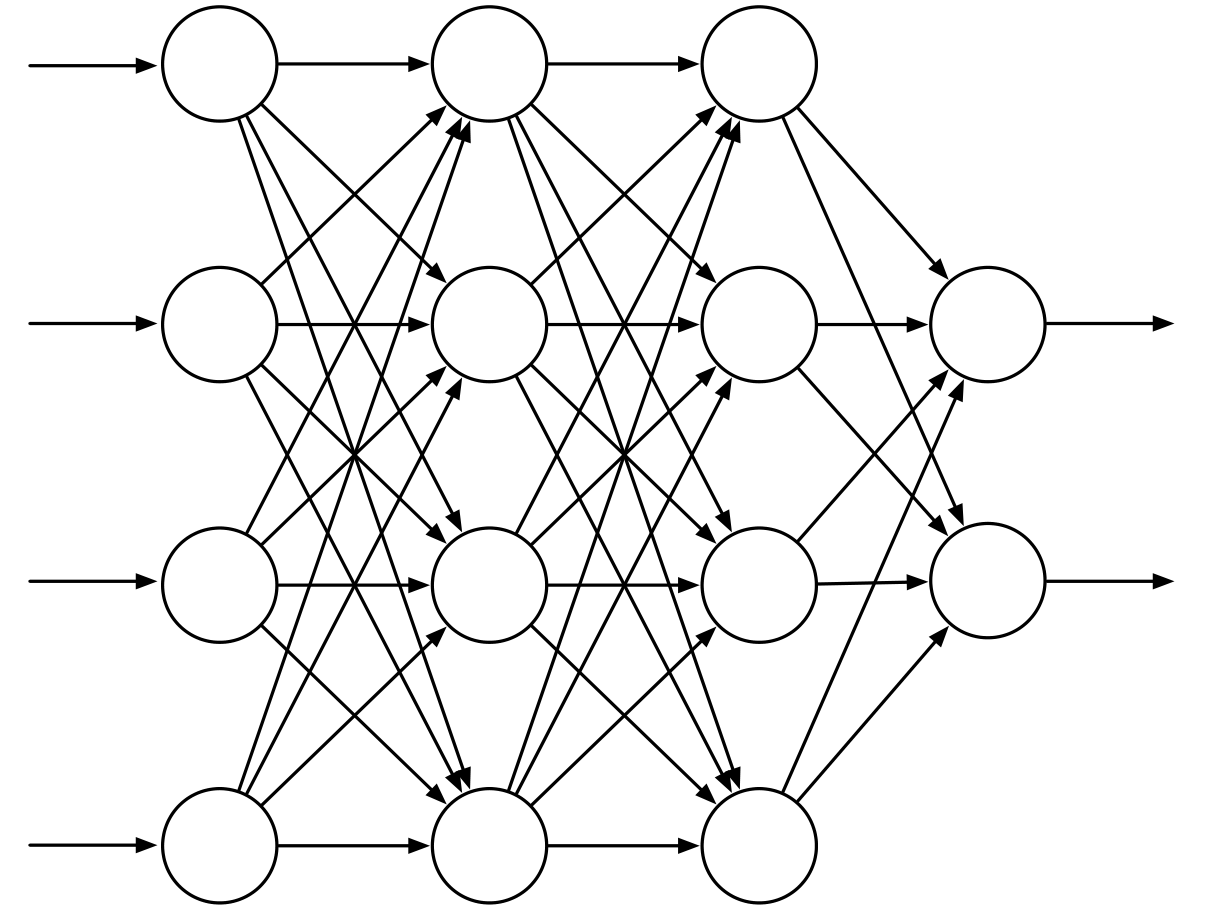
\includegraphics[width=0.95\linewidth]{./fig/ann.png}
\caption[Artificial Neural Network]{A sample ANN consisting of four input nodes, two fully connected hidden layers and two output nodes \cite{sutton18_reinf}. \protect\footnotemark \label{fig-ann}}
\end{figure}
\footnotetext{\textbf{Figure 9.14} from "Reinforcement Learning: An Introduction" by Richard S. Sutton and Andew G. Barto is licencsed under CC BY-NC-ND 2.0 (https://creativecommons.org/licenses/by-nc-nd/2.0/)}
\subsubsection{Further Topics}
\label{sec:orgb9f00e3}
The previous chapters provided a detailed overview of the most important
concepts and mathematical foundations in RL. In the research there are many more
topics that were not covered here. \emph{Eligibility traces} offer a way to more
general learning and faster convergence rates. Almost any TD method can be
extended to use eligibility traces, a popular methods is called Watkins's Q(\(\lambda\))
\cite{watkins89_learn_from_delay_rewar}. \emph{Fitted-Q Iteration} \cite{ernst03_iterat}
combined Q-learning and fitted value iteration with batch-mode RL. In
batch-mode the whole dataset is available offline, contrary to online RL where
the data is acquired by the agent's action in its the environment.
\emph{Actor-critic} methods \cite{sutton84_tempor_credit_assig_reinf_learn} directly
learn a parameterized policy instead of action-values, which inherently allow
continuous state spaces and learning appropriate levels of exploration.
Simultaneously to learning the policy, they approximate a state-value function,
which serves as a "critic" to the learned policy, the "actor". In the current
theory most RL models are single-agent models. For certain real-world
applications multi-agent RL algorithms are necessary to coordinate interaction
between the agents. When multiple learning agents interact with a non-stationary
environment, convergence and stability are a serious problem. \emph{W-learning}
\cite{humphrys96_action_selec_method_using_reinf_learn} is an multi-agent approach
that aims to solve these difficulties.

\clearpage
\section{Empirical Setting}
\label{sec:orgf7ebb94}
This research is embedded in the German carsharing and electricity markets.
Germany is a suitable testbed, since it has a comparably high share of
renewables in its energy mix and is pushing for an energy turnaround (German:
\emph{Energiewende}) since 2010 \cite{bmu10_energ_concep_envir_sound_reliab_affor}
The high renewable energy content in the energy mix causes electricity prices to
be volatile, which makes Germany an attractive location for the use of
VPPs.

Germany is home to the carsharing providers Car2Go\footnote{\url{https://www.car2go.com}} and DriveNow\footnote{\url{https://www.drive-now.com}},
which operate large EV fleets across the globe. It has been argued that electric
carsharing can simultaneously solve several traditional mobility and
environmental problems and are an important element of future smart cities
\cite{firnkorn15_free_float_elect_carsh_fleet_smart_cities}. Further, it is widely
regarded that the future of mobility will be electric, shared, smart and
eventually autonomous \cite{burns13_sustain_mobil,sterling18_three_revol}.
Carsharing providers are already contributing to the first two points by
operating large fleets of electric vehicles. This research addresses the third
point: Using electric carsharing fleets to smartly participate in electricity
markets. Carsharing providers, like Car2Go and DriveNow, operate their
carsharing fleets in a free-float model, which allows customers to pick up and
drop vehicles at any place within the operating zone of the provider. Customers
pay by the minute and are offered incentives to park the EVs at charging
stations at the end of their trip.

We obtained real-world trip data from Daimler's carsharing service Car2Go.
Additionally, we collected freely available balancing market data from the GCRM
platform website \url{https://regelleistung.net}. The data of the EPEX Spot market
have kindly been provided by ProCom GmbH\footnote{\url{https://procom-energy.de}} for research purposes. In the
next chapters the different datasets are described, as well the most important
processing steps outlined.

\subsection{Electronic Vehicle Fleet Data}
\label{sec:orgab93a92}
The Car2Go dataset consists of GPS data of around 500 Smart ED3 Fortwo vehicles in
Stuttgart. These subcompact cars are equipped with a 17.6kWh battery and a
standard 3.3kW on-board charger. They fully charge in about six to seven hours
and can reach a maximum driving distance of 145km according to the manufacturer.
When equipped with an additional 22kW fast charger the charging time reduces to
about an hour.

In Table \ref{table-car2go-raw} the raw data is displayed, as we have obtained it
by Car2Go. The dataset contains spatio-temporal attributes, such as timestamp,
coordinates, and the address of the EVs in 5 minute intervals. Additionally,
status attributes of the interior and exterior are given (not displayed).
Especially relevant for our research is the state of charge (\(SoC\), in \%) and
information whether the EV is plugged into one of the 380 charging stations in
Stuttgart. Note that the data only contain EVs that are \emph{available for rent},
i.e., they are not currently rented out by a customer. EVs which are parked at a
charging station are also not available until they have charged up approximately
70 SoC. Individual trips have to be reconstructed using the GPS data of the
cars. The following preprocessing steps have been taken to prepare the data for
further analysis. Table \ref{table-car2go-processed} depicts the dataset after all
processing steps.

\begin{enumerate}
\item Drop unused data columns

\begin{itemize}
\item \emph{ID}: Number plate is already a unique identifier for every EV.
\item \emph{Address}: Different addresses were given from same coordinates. \emph{Latitude,
Longitude} was used for locational data instead.
\item \emph{Interior, Exterior}: Status attributes were not used in the analysis of
this research. Although they could form interesting features for rental
predictions.
\item \emph{Engine Type}: All EVs in Stuttgart are electric vehicles.
\end{itemize}
\item Decrease GPS resolution to 10 meters

The GPS accuracy of private industry sensors is approximately 5 meters under
open sky, and worse near buildings, bridges and trees\footnote{See \url{https://www.gps.gov/systems/gps/performance/accuracy}, accessed
23\textsuperscript{th} February 2019.}. Rental trips are
identified by changing GPS locations of the EV (See next point). To reduce
the number of false identified trips, due to GPS measurement errors, the resolution
is decreased.
\item Determine rental trips

We infer that a customer rented a EV, if the position coordinates change
between two data points of the same EV (see Table \ref{table-car2go-raw}, 4\textsuperscript{th}
to 5\textsuperscript{th} row). Note that we assume that customer do not undertake trips,
which begin and end at the exact same location.
\item Infer charging stations

The GPS location of the EVs is matched with the GPS locations, where an EV
has been charged at least once in the dataset. We observed that the raw data
do not show EVs that are parked at charging stations, but are not plugged in.
This research assumes that all EVs, which are parked at charging stations are
also plugged in. That is a valid assumption, since in Germany cars are only
allowed to park at charging station if they are connected to it.
\item Clean data
\begin{itemize}
\item \emph{Service trips}: 999 rental trips were removed that had a trip duration
longer than the maximum allowed rental time of two days. We assume that
these trips were \emph{service trips} undertaken by Car2Go. When the EVs
returned with a higher SoC (e.g., they have been charged at the car repair
shop), the previous trip had to be altered to end at a charging station to
ensure charging consistency.
\item \emph{Incorrectly charged EVs}: 999 EVs were removed that show incorrect
charging behavior. The data of these EVs showed an increase of more than
20\% SoC between trips or on trips, while not being located at a charging
station.
\end{itemize}
\end{enumerate}

\begin{sidewaystable}[htbp]
    \caption{Sample Raw Car2Go Data in Stuttgart \label{table-car2go-raw}}
    \centering
    \begin{tabular}{c|ccccccc}
      \hline
      \hline
      Number Plate & Timestamp & Latitude & Longitude & Street & Zip Code & Charging & SoC (\%)\\
      \hline
      S-GO2471 & 24.12.2017 20:00 & 9.19121 & 48.68895 & Parkplatz Flughafen & 70692 & no & 94\\
      S-GO2471 & \ldots{} & \ldots{} & \ldots{} & \ldots{} & \ldots{} & \ldots{}. & \ldots{}\\
      S-GO2471 & 24.12.2017 20:05 & 9.19121 & 48.68895 & Parkplatz Flughafen & 70692 & no & 94\\
      S-GO2471 & 24.12.2017 20:10 & 9.19121 & 48.68895 & Parkplatz Flughafen & 70692 & no & 94\\
      S-GO2471 & 24.12.2017 23:05 & 9.15922 & 48.78848 & Salzmannweg 3 & 70192 & no & 71\\
      S-GO2471 & 24.12.2017 23:10 & 9.15922 & 48.78848 & Salzmannweg 3 & 70192 & no & 71\\
      S-GO2471 & 25.12.2017 00:40 & 9.17496 & 48.74928 & Felix-Dahn-Str. 45 & 70597 & yes & 62\\
      S-GO2471 & 25.12.2017 00:45 & 9.17496 & 48.74928 & Felix-Dahn-Str. 45 & 70597 & yes & 64\\
      S-GO2471 & \ldots{} & \ldots{} & \ldots{} & \ldots{} & \ldots{} & \ldots{}. & \ldots{}\\
      S-GO2471 & 25.12.2017 06:50 & 9.17496 & 48.74928 & Felix-Dahn-Str. 45 & 70597 & no & 100\\
      S-GO2471 & 25.12.2017 08:25 & 9.2167 & 48.78742 & Friedenaustraße 25 & 70188 & no & 42\\
      \hline
      \hline
    \end{tabular}

    \bigskip\bigskip  % provide some separation between the two tables

    \caption{Sample Processed Car2Go Trip Data in Stuttgart \label{table-car2go-processed}}
    \centering
    \begin{tabular}{cc|ccccc}
      \hline
      \hline
      Number Plate & Trip & Start Time & Start Latitude & Start Longitude & Start SoC (\%)\\
      \hline
      S-GO2471 & 1 & 24.12.2017 20:10 & 9.19121 & 48.68895 & 94\\
      S-GO2471 & 2 & 24.12.2017 23:10 & 9.15922 & 48.78848 & 71\\
      S-GO2471 & 3 & 25.12.2017 00:50 & 9.17496 & 48.74928 & 66\\
      \hline
      Number Plate & Trip & End Time & End Latitude & End Longitude & End SoC (\%)\\
      \hline
      S-GO2471 & 1 & 24.12.2017 23:05 & 9.15922 & 48.78848 & 71\\
      S-GO2471 & 2 & 25.12.2017 00:40 & 9.17496 & 48.74928 & 62\\
      S-GO2471 & 3 & 25.12.2017 03:25 & 9.2167 & 48.78742 & 42\\
      \hline
      Number Plate & Trip & Trip Duration (min) & Trip Distance (km) & Trip Charge (\%) & End Charging\\
      \hline
      S-GO2471 & 1 & 175 & 33.35 & 23 & no\\
      S-GO2471 & 2 & 90 & 13.05 & 9 & yes\\
      S-GO2471 & 3 & 155 & 29 & 20 & no\\
      \hline
      \hline
    \end{tabular}
\end{sidewaystable}

\subsection{Balancing Market Data}
\label{sec:orgb9ec0b5}
In this research, we use market balancing data from the German secondary reserve
market. The following chapter will give an overview of the dataset and
preprocessing steps that were taken. The data encompasses weekly lists of
anonymized bids between 01.06.2016 and 01.01.2018 and a dataset of activated
control reserve in Germany during the same period. For a detailed description
about the market design of balancing markets refer to Chapter
\ref{sec-balancing-market}.

The bidding data consists of the traded electricity product, the offered
capacity \(\Pb{}\) (MW), the capacity price \(\cp{}\) (\(\text{\euro{}/MW}\)), and the
energy price \(\ep{}\) (\(\text{\euro{}/MWh}\)) of each bid. Four different products
are traded, which are a combination of positive control reserve (feed
electricity into the grid) or negative control reserve (take electricity from
the grid) and the provided time segment (peak or non-peak hours). Since negative
prices are allowed on the secondary operating reserve market, the payment
direction is included as well. Moreover, information about the amount of
capacity that was accepted, i.e., either partially or fully, is listed. Bids,
which were not accepted by the TSOs are not listed. An exemplary excerpt of the
dataset is displayed in Table \ref{table-operating-reserve}.

\begin{longtable}{c|ccccc}
\caption[Secondary Operating Reserve Market Data]{List of Bids of the German Secondary Reserve Market for the tender period 04.12.2017 - 11.12.2017. \label{table-operating-reserve}}
\\
\hline
\hline
Product & Capacity Price & Energy Price & Payment & Offered & Accepted\\
\hline
\endfirsthead
\multicolumn{6}{l}{Continued from previous page} \\
\hline

Product & Capacity Price & Energy Price & Payment & Offered & Accepted \\

\hline
\endhead
\hline\multicolumn{6}{r}{Continued on next page} \\
\endfoot
\endlastfoot
\hline
NEG-HT & 0 & 1.1 & TSO to bidder & 5 & 5\\
NEG-HT & 10.73 & 251 & TSO to bidder & 15 & 15\\
NEG-HT & 200.3 & 564 & TSO to bidder & 22 & 22\\
\ldots{} & \ldots{} & \ldots{} & \ldots{} & \ldots{} & \ldots{}\\
NEG-NT & 0 & 21.9 & Bidder to TSO & 5 & 5\\
NEG-NT & 0 & 22.4 & Bidder to TSO & 5 & 5\\
\ldots{} & \ldots{} & \ldots{} & \ldots{} & \ldots{} & \ldots{}\\
POS-NT & 696.6 & 1200 & TSO to bidder & 5 & 5\\
POS-NT & 717.12 & 1210 & TSO to bidder & 10 & 7\\
\hline
\hline
\end{longtable}

In this study, we assume that bidding on 15-minute intervals in secondary
operating reserve auctions will be possible in future energy markets. As
mentioned in Chapter \ref{sec-balancing-market}, the market design of the GCRM
secondary operating reserve tender was adjusted in 2017. Daily tenders with
4-hour bidding intervals were introduced in favor of weekly tenders with only
two time segments. This change represents the trend by the TSOs to change the
market design in order to better include RES into the operating reserve markets
\cite{agricola14_dena_ancil_servic_study}. Due to the volatility of renewable
electricity generation, providers are naturally dependent on accurate short-term
forecasts, which are only possible with short tender periods and fine-grained
bidding intervals.

In order to estimate the upper bound of profits that the EV fleet can earn by
participating in the secondary operating reserve market, the \emph{critical prices}
\(\ccp{}\) and \(\cep{}\) were determined for each auctioned interval. Following
\textcite{brandt17_evaluat_busin_model_vehic_grid_integ}, we define \(\ccp{}\)
(\(\text{\euro{}/MW}\)) as the capacity price of the bid that was just barely
accepted, whereas \(\cep{}\) (\(\text{\euro{}/MWh}\)) is the highest energy price
that was payed for activated control reserve during that interval. For every
15-minute interval within the given tender period of one week, the activated
control reserve in that interval was matched with the accepted bids in that
tender period. At the point where supply, i.e., offered capacity of bids, met
demand, i.e., activated control reserve, the critical price \(\cep{}\) was
determined.

\emph{Example}: The assumed critical prices for the secondary operating reserve
tender interval of the 6\textsuperscript{th} December 2017 between 08:00 and 08:15 are obtained
as follows: Three suppliers submitted a reserve capacity of 5MW, 15MW and 22MW
respectively (see Table \ref{table-operating-reserve}). The critical capacity
price \(\ccp{} = 200.3 \text{ \!\euro{}/MW}\) is determined by the
capacity price of the last (third) accepted bid in that time segment. The TSO
reported that 18MW of control reserve were activated between 08:00 and 08:15.
Hence, the second bid determines the critical energy price \(\cep{} = 251
\text{ \!\euro{}/MWh}\), as control reserve capacity gets activated according to
ascending order of the submitted energy prices. In this example the second
bidder would get compensated with: \(R = R^c + R^e =(10.73
\text{ \!\euro{}/MW}\times15\text{MW}) + (251
\text{ \!\euro{}/MWh}\times13\text{MW}\times 0.25\text{h}) =
976.7\text{ \!\euro{}}\). Note that the second bidder get compensated for
providing 13MW for 15 minutes (0.25h), instead of the submitted 15MW, since in
total only 18MW of control capacity was activated, which was partly fulfilled
by the 5MW of the first bidder.

\subsection{Spot Market Data}
\label{sec:org8b81ca2}
The data from the EPEX Spot Intraday Continuous encompass order books and
executed trades from 01.06.2016 until 01.01.2018. The list of trades contain
information on the unit price \(\up{}\) (\(\text{\euro{}/MWh}\)), the quantity \(Q\)
(kW) and the traded product (hourly, quarterly or block). In this research, we
focus on quarterly product times (15-minute intervals), as they provide the
highest flexibility. Fleet controllers can promptly react to fluctuant
electricity demand of the EV fleet by accurately adjusting the bid quantities.
Future research could also consider other electricity products if lower prices
justify decreased flexibility at that point in time. Additionally, the TSOs of
the buyer and seller are listed in the dataset. They are only relevant if
special conditions between TSO apply, e.g., when delivering electricity to other
countries.

On the spot market, electricity trades can have a very short lead time of up to
5 minutes before delivery (see Table \ref{table-spot-market}). This market
characteristic is beneficial for our proposed trading strategy, since it allows
the EV to procure electricity in almost real time. The controller can submit
bids to the market, with accurate estimations of available charging capacity up
to five minute-ahead. Similarly to the balancing market, the critical price
\(\cup{}\) has to be determined for all intraday trading intervals.
\(\cup{}\) is defined as the lowest unit price of all executed trades
\(\cal{T}\) in a bidding interval:
\begin{equation*}
    \cup{} \defeq \min_{t \in \cal{T}} \up{t}
\end{equation*}
Note that \(\cup{}\) is essentially the optimal bidding price, it provides
on upper bound for the fleets profits when bidding on the intraday market. We
assume that bids with  \(p_u \geq \cup{}\) will always get matched. In
reality this is not always the case, since trades are executed immediately and
it is not guaranteed that unmatched asks at \(\cup{}\) exist at the time
of commitment. For a detailed description of the intraday continuous market see
Chapter \ref{sec-spot-market}.

{\captionsetup[table]{aboveskip=0.5cm}
\begin{sidewaystable}[hp]
\caption{List of Trades of the EPEX Spot Intraday Continuous Market \label{table-spot-market}}
\centering
\begin{tabular}{c|cccccccc}
\hline
\hline
Execution time & ID & Unit Price & Quantity & Buyer Area & Seller Area & Product & Product Time & Delivery Date\\
\hline
2017-12-04 06:54:55 & 8031392 & 51.00 & 5500 & Amprion & Amprion & Q & 07:15 - 07:30 & 2017-12-04\\
2017-12-04 06:53:26 & 8031391 & 59.00 & 10000 & TenneT & TenneT & Q & 07:15 - 07:30 & 2017-12-04\\
2017-12-04 06:53:26 & 8031390 & 58.90 & 10000 & TenneT & TenneT & Q & 07:15 - 07:30 & 2017-12-04\\
2017-12-04 06:53:15 & 8031389 & 52.30 & 7000 & 50Hertz & 50Hertz & Q & 07:15 - 07:30 & 2017-12-04\\
2017-12-04 06:53:13 & 8031386 & 59.00 & 500 & TenneT & TenneT & Q & 07:15 - 07:30 & 2017-12-04\\
2017-12-04 06:53:13 & 8031387 & 51.00 & 3600 & Amprion & Amprion & Q & 07:15 - 07:30 & 2017-12-04\\
2017-12-04 06:53:13 & 8031388 & 52.00 & 1400 & Amprion & Amprion & Q & 07:15 - 07:30 & 2017-12-04\\
2017-12-04 06:53:02 & 8031385 & 58.90 & 11000 & TenneT & TenneT & Q & 07:15 - 07:30 & 2017-12-04\\
2017-12-04 06:52:38 & 8031380 & 60.00 & 10000 & Amprion & Amprion & Q & 07:15 - 07:30 & 2017-12-04\\
2017-12-04 06:52:38 & 8031381 & 57.50 & 8000 & Amprion & Amprion & Q & 07:15 - 07:30 & 2017-12-04\\
2017-12-04 06:52:38 & 8031382 & 58.00 & 2000 & Amprion & Amprion & Q & 07:15 - 07:30 & 2017-12-04\\
2017-12-04 06:52:38 & 8031383 & 58.90 & 4000 & TenneT & TenneT & Q & 07:15 - 07:30 & 2017-12-04\\
2017-12-04 06:52:38 & 8031384 & 60.00 & 4000 & Amprion & Amprion & Q & 07:15 - 07:30 & 2017-12-04\\
2017-12-04 06:52:27 & 8031379 & 52.30 & 8000 & 50Hertz & 50Hertz & Q & 07:15 - 07:30 & 2017-12-04\\
2017-12-04 06:51:33 & 8031378 & 66.00 & 5000 & TransnetBW & TransnetBW & Q & 07:15 - 07:30 & 2017-12-04\\
2017-12-04 06:51:28 & 8031377 & 54.00 & 8000 & Amprion & Amprion & Q & 07:15 - 07:30 & 2017-12-04\\
2017-12-04 06:51:24 & 8031376 & 54.00 & 7000 & TenneT & TenneT & Q & 07:15 - 07:30 & 2017-12-04\\
2017-12-04 06:49:34 & 8031375 & 51.00 & 4000 & TenneT & TenneT & Q & 07:15 - 07:30 & 2017-12-04\\
2017-12-04 06:49:26 & 8031374 & 54.00 & 5000 & 50Hertz & 50Hertz & Q & 07:15 - 07:30 & 2017-12-04\\
2017-12-04 06:49:23 & 8031373 & 55.10 & 8000 & 50Hertz & 50Hertz & Q & 07:15 - 07:30 & 2017-12-04\\
\hline
\hline
\end{tabular}
\end{sidewaystable}
}

\clearpage
\section{Model: FleetRL}
\label{sec:orgccacf48}
The following chapter will introduce the model of this research. In its essence,
we propose a solution for EV fleet providers to utilize a portfolio of VPPs to
profitably provide balancing services to the grid on multiple markets. A control
mechanism procures energy from electricity markets, allocates available EVs to
VPPs, and intelligently dispatches EVs to charge the acquired amount of energy.
The model uses a RL agent that learns an optimal bidding strategy by interacting
with the electricity markets and reacts to changing rental demand of the EV
fleet. This chapter is structured as follows: First, the information assumptions
are listed, and the general control mechanism is explained. Afterwards, the
bidding strategy and the RL approach are described in detail. Finally, the
dispatch algorithm is presented.

We formulate the problem as a \emph{controlled EV charging} problem. The EV fleet
operator represents the \emph{controller}, which aims to optimally charge the fleet
by providing balancing capacity. First, the controller predicts the amount of
energy it can charge in a given \emph{market period} \(h\). The length of the market
period \(\Delta h\) and the market closing time depend on the considered
electricity market. Second, the controller places bids on one or multiple
markets to procure the predicted amount of energy. Lastly, at electricity
delivery time, the controller communicates with the EV fleet to control the
charging in real-time. Online EV \emph{control periods} \(t\) are typically shorter
than market periods. In our case, the market periods of the considered markets
are 15 minutes long, while we consider EV control periods of 5 minutes. During
each control period, the controller has to take decisions about dispatching
individual EVs for charging according to a heuristic function \(f_{heur}\). In
times of unforeseen rental demand, this decision implies trading off commitments
to the markets with compromising customer mobility by refusing customer rentals.

\begin{longtable}{l|p{0.7\linewidth}|l}
\caption[Table of Notation]{Table of Notation \label{table-notation}}
\\
\hline
\hline
Variable & Description & Unit\\
\hline
\endfirsthead
\multicolumn{3}{l}{Continued from previous page} \\
\hline

Variable & Description & Unit \\

\hline
\endhead
\hline\multicolumn{3}{r}{Continued on next page} \\
\endfoot
\endlastfoot
\hline
\(t\) & Control period. & -\\
\(h\) & Market period. & -\\
\(T\) & Total number of control periods in day. & -\\
\(H\) & Total number of market periods in day. & -\\
\(\Delta t\) & Length of control period. & minutes\\
\(\Delta h\) & Length of market period. & minutes\\
\(N_t\) & Number of control periods in a market period. & -\\
\hline
\(\Pb{h}\) & Amount of power offered on the balancing market. & kW\\
\(\cp{h}\) & Capacity price offered on the balancing market. & \(\text{\euro{}/MW}\)\\
\(\ep{h}\) & Energy price offered on the balancing market. & \(\text{\euro{}/MWh}\)\\
\(\ccp{h}\) & Critical capacity price in market period \(h\). & \(\text{\euro{}/MW}\)\\
\(\cep{h}\) & Critical energy price in market period \(h\). & \(\text{\euro{}/MWh}\)\\
\hline
\(\Pi{h}\) & Amount of power offered on the intraday market. & kW\\
\(\up{h}\) & Unit price offered on the intraday market. & \(\text{\euro{}/MWh}\)\\
\(\cup{h}\) & Critical unit price in market period \(h\). & \(\text{\euro{}/MWh}\)\\
\hline
\(\Eb{h}\) & Amount of energy charged from balancing market in market period h. & MWh\\
\(\Ei{h}\) & Amount of energy charged from the intraday market in market period h. & MWh\\
\hline
\(\fQ{t}\) & Amount of available fleet charging capacity in control period \(t\). & kWh\\
\(\fP{t}\) & Amount of available fleet charging power in control period \(t\). & kW\\
\(\fPhat{t}\) & Predicted amount of available fleet charging power in control period \(t\). & kW\\
\hline
\(p^{i}\) & Industry tariff & \(\text{\euro{}/MW}\)\\
\(\fh\) & Heuristic function to dispatch EVs to charging & -\\
\hline
\hline
\end{longtable}

\subsection{Required Information Assumptions}
\label{sec:org2db7e5a}
In order to optimize the controller's bidding strategy, the following
information is assumed to be available:

\begin{enumerate}
\item The controller is able to forecast the mobility demand of the EV fleet at
different time-horizons based on historical data. More specifically, it can
predict the amount of plugged-in EVs and consequently the charging
power \(P^{fleet}_t\) of the fleet at control period \(t\). The prediction's
accuracy is increasing with shorter time horizons, from one week, 24 hours to
30 minutes ahead. Past research presented successful mobility demand forecast
algorithms in the context of free-float carsharing
\cite{kahlen18_elect_vehic_virtual_power_plant_dilem,kahlen17_fleet,wagner16_in_free_float}.
\item The controller is able to forecast electricity prices of spot and balancing
markets based on historical data. More specifically, it can estimate the
critical prices \(\ccp{h}\), \(\cep{h}\), and \(\cup{h}\) for each market period
with perfect accuracy. The critical prices form an essential piece of
information for the proposed bidding strategy; bids equal or below the
critical price result in successful procurement. Electricity price
forecasting is an  extensively studied research area, with well-advanced
prediction algorithms
\cite{weron14_elect_price_forec,avci18_manag_elect_price_model_risk}.
\end{enumerate}
We are confident that taking the above assumptions is viable, assuming available
forecasting information is common practice in the VPP and EV fleet charging
literature
\cite{brandt17_evaluat_busin_model_vehic_grid_integ,vandael15_reinf_learn_heuris_ev_fleet,mashhour11_biddin_strat_virtual_power_plant_1,tomic07_using_fleet_elect_drive_vehic_grid_suppor}.

\subsection{Control Mechanism}
\label{sec:orgb9e0696}
The central control mechanism constitutes the core of this research. It can be
seen as a decision support system that can be employed at a EV fleet operator to
facilitate smart charging its fleet. The control mechanism is divided into three
distinct phases (see Figure \ref{fig-control-mechanism}).

\begin{figure}[htbp]
\centering
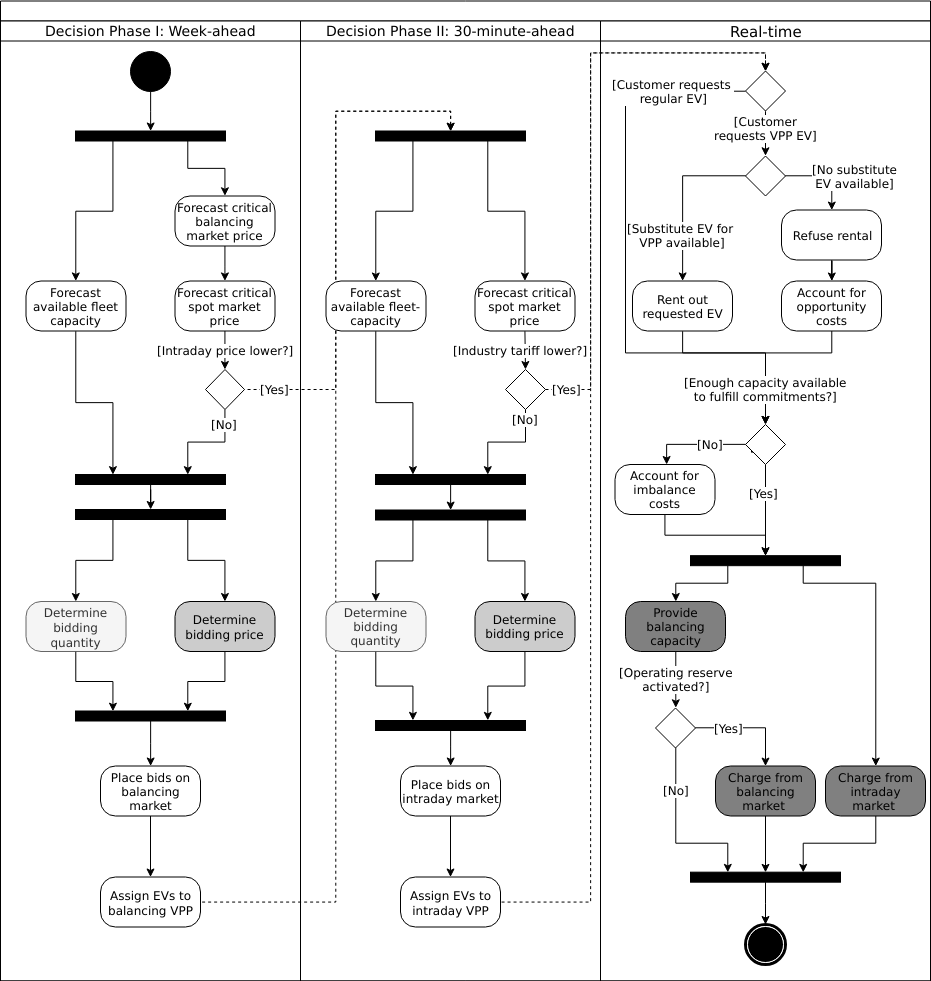
\includegraphics[width=1\linewidth]{./fig/control_mechanism.png}
\caption[EV VPP Control Mechanism]{EV VPP Control Mechanism \label{fig-control-mechanism}}
\end{figure}

\subsubsection{Decision Phase I: Week ahead}
\label{sec:org17f3067}
The first decision phase occurs just before the closing time of the balancing
market, once every week (e.g., Wednesdays at 3pm at the GCRM). In this phase, the
controller can place bids for every market period \(h\) of the following week on
the balancing market. When a bid gets accepted, the fleet has to provide the
committed charging capacity during all control periods \(t\) of the market period
\(h\). In order to optimally place bids on the balancing market the controller has
to take the following steps:

First, the controller has to predict the available fleet charging power \(\fP{h +
(H \times 7)}\) one week ahead, where \(H\) is the number of market periods in a
day. To minimize the risk of not being able to provide the committed capacity,
and consequently causing imbalance costs, the predicted fleet charging power in
a market period is defined as the minimal predicted fleet charging power in the
control periods that make up the market period (\(N_t\)).
\begin{equation}
    \fPhat{h} \defeq \min_{n \in \{1, .., N_t\}} \fPhat{t + n} \text{ ,}
\end{equation}
where \(h\) is the market period of interest and \(t\) its first control period.

Second, the controller has to decide from which market it should procure the
desired amount of energy. Therefore, it compares the costs for charging from the
balancing and intraday market.  As mentioned in the previous section, the
critical prices \(\ccp{}, \cep{}, \cup{}\) are assumed to be available for all
market periods. The cost function for charging from the balancing market is
defined as follows:
\begin{equation} \label{eq-cost-balancing}
\begin{split}
    \Cb{h}(P) &\defeq  -(P  \times \ccp{h}) + (\Eb{h} \times \cep{h}) \\
    &= -(P  \times \ccp{h}) + (P \frac{\Delta h}{60} \times \cep{h}) \text{ ,}
\end{split}
\end{equation}
where \(P\) is the amount of power charged in kW. The first term of the equation
corresponds to the compensation the controller retrieves for keeping the
balancing capacity available, while the second term corresponds to the costs for
charging the activated balancing energy \(\Eb{h}\). Energy is the delivered power
over time, hence \(\Eb{h}\) can be substituted with the \(P\) times the  market
periods fraction of an hour \(\frac{\Delta h}{60}\). Note that the critical energy
price \(\cep{}\!\in\!\Re\), can also take negative values, resulting in profits
for the fleet, while the critical capacity price \(\ccp{}\!\in\! \Re^+_0\) is
always greater than zero and thus never results in costs for the fleet. The cost
function for charging from the intraday market is defined similarly to Equation
(\ref{eq-cost-balancing}):
\begin{equation}
\begin{split}
    \Ci{h}(P) &\defeq \Ei{h} \times \cup{h} \\
    &= P \frac{\Delta h}{60} \times \cup{h} \text{ ,}
\end{split}
\end{equation}
Again, depending on the market situation, \(\cup{}\!\in\!\Re\) can be either
negative or positive, resulting in costs or profits for the fleet. Contrarily to
the balancing market, on the intraday market the fleet does not get compensated
for keeping the charging power available. When the costs for charging from the
balancing market one week ahead \(\Cb{h + (H \times 7)}(\fPhat{h + (H \times
7)})\) are higher than the costs of charging from the intraday market at the same
market period \(\Ci{h + (H \times 7)}(\fPhat{h + (H \times 7)})\), the controller
does not place bids on the balancing market and continues to Decision Phase II.

Third, the controller has to take a decision on the amount of charging power
it should submit to the balancing market. Determining the bidding quantity is a
central piece of the controlled charging problem. The controller needs to
balance the risks of

\begin{enumerate}
\item Not committing enough power to the market and thus not charging the fleet enough
\item Committing more power that it can deliver and thus facing costs
\begin{itemize}
\item Opportunity cost of compromising customer mobility. Renting EVs is more
profitable than using the EV for VPP activities. Refunsing customer rentals
\end{itemize}
\end{enumerate}

by foregone rentals, when trips are refused for the sake
     of VPP
\begin{itemize}
\item
\end{itemize}
imbalance costs or compromising customer mobility with profits that can be made
from charging at a cheaper price than industry tariff. Because \(f\fPhat{}\) faces
uncertainty with increasing time, the controller also has to weigh balancing vs
intraday\ldots{}

\begin{equation}
\Pb{h} = \fPhat{h} - \lambda_{h}
\end{equation}

\begin{enumerate}
\item Light-grey: Determine bidding quantity, Chapter \ref{sec-model-rl}
\begin{itemize}
\item Essential Information, determines Smart Charging quantities.
\item Balance risks versus profits
\item Need to have sufficient SoC to be able to rent out. Not enough SoC violates
customer mobility, and thus decreases profits
\item Conflicting: Do not submit/charge too much: When no replacement for VPP is
available, we loose rental profits and also violate customer mobility
\item Conflicting: Do not submit quantities we can not charge. Causes high
imbalance costs that have to be avoided at all times
\item RL Agent!
\end{itemize}
\item Middle-grey: Determine bidding price \ref{sec-model-bidding-strategy}
\end{enumerate}


\(T(h)\) Mapping from market period \(h\) to the set of control periods in market
period \(h\).

Nomenclature:
\begin{itemize}
\item Use Notion of consumption plan?
\end{itemize}

Figure:
\begin{itemize}
\item What about regular charging?
\item What about not enough SoC for trip?
\item Allocate costs/profits from charging/trip?
\item Other figure, with timely bidding and control periods?
\end{itemize}

Assume:
\begin{itemize}
\item Operating reserve always gets activated.
\item Bid at \(p_c = 0\)
\item EVs charge at industry tariff, when not allocated to VPP
\item Bid always multiples of charging capacity, do not consider charging at
different speeds
\end{itemize}

Mechanism:
\begin{itemize}
\item Only EVs with enough battery capacity left to charge the next control period
are allocated to VPP.
\end{itemize}

Other assumptions:
\begin{enumerate}
\item Bids on balancing market always get accepted (Known critical capacity price \(\ccp{}\)
\item EV fleet charges at a fixed industry tariff otherwise
\item Balancing capacity is provided for a market period \(h\). Within the market
period \(h\), it is possible to provide the capacity with different EVs,
changing in control periods \(t\). Customers arrive in \(t\) intervals.
\end{enumerate}

Ideas:
\begin{itemize}
\item What about imbalance costs that can be bough/sold from other market like in
\cite{vandael15_reinf_learn_heuris_ev_fleet}? \(\lambda_h^+\): Less energy charged
than bought at electricity prices, EV Fleet controller gets refunded based on
a positive imbalance price \$\(\lambda\)\textsubscript{h}\^{}+ < \(\up{}\). Because positive imbalance
prices are lower than charging prices, only partially refunded for excess
energy bought in electricity markets.

\item Mathematical notation for foregone rentals!
\end{itemize}


\subsubsection{Decision Phase II: 30 Minutes ahead}
\label{sec:orgdf79067}
\subsubsection{Dispatch Phase: Real-time}
\label{sec:orgf91d35f}

\begin{itemize}
\item \(f_{heur}\) Heuristic function to dispatch power to EVs
\end{itemize}


\subsection{(Fleet Capacity \& Critical Price Prediction)}
\label{sec:org295b012}
\begin{itemize}
\item Fleet capacity prediction made on non-simulated real-world SoC (w/o smart charging)
\begin{itemize}
\item Provide difference levels \& descriptive statistics?
\item Already enough uncertainty or artificially add more?
\item Balancing forecasts needs more uncertainty than intraday, otherwise RL does
not make sense: Handle uncertainty.
\item Prediction:
\begin{itemize}
\item Predict for all c in h
\item Q = min(q\textsubscript{c})
\end{itemize}
\end{itemize}

\item Electricity prices:
\begin{itemize}
\item Artificially add uncertainty to prediction by distorting real-world data
according to Gaussian distribution
\end{itemize}
\end{itemize}

\subsection{Bidding Strategy \label{sec-model-bidding-strategy}}
\label{sec:org1d0a7c1}
Assumptions:
\begin{itemize}
\item EV fleet is price taker, it is lacking the market share to influence prices
\begin{itemize}
\item \(\rightarrow\) Use existing prices
\end{itemize}
\item Relax minimum bidding assumption of 1MW to no limit. Sensitivity analysis
with 100kw and 500kw in evaluation
\item Controller always bids at an optimal price.
\end{itemize}

intraday:
\begin{equation}
\begin{split}
    b^{intr} &= (P^{intr}, p_u) \\
    p_u &= \min(\cup{}, p_r) \\
    P^{intr} &= \pi(s)
\end{split}
\end{equation}

balancing:
\begin{equation}
\begin{split}
    b^{bal} &= (P^{bal}, p_c, p_w) \\
    P^{bal} &= \pi(s) \\
    p_c &= 0 \\
    p_w &= \min(\overline{p_w}, p_r)
\end{split}
\end{equation}

\begin{itemize}
\item Optimal price
\item Forecasted critical prices. Different accuracy levels?
\item Use critical prices - threshold? Or
\item Assume always the perfect bid: Upper-bound evaluation
\item Compare with industry-tariff
\item Figure about prices over the day? Compare
\item What about balancing capacity prices? Future work?
\item Mathematical formulation
\end{itemize}

Furthermore, we assume the
aggregator is a price-taker. In case of limited size purchase
orders, an aggregator will naturally have a price-taker position.

The fleet controller offers bids and asks for every time interval. These offers
contain both a quantity and a reservation price, which depends on the state of
charge of the EV storage, as well as on the battery costs. However, the market
may or may not accept these offers depending on the composition of the offer
prices from the fleet owner and other market participants. The market auction
mechanism ultimately decides when EVs will charge and discharge.

\subsection{Reinforcement Learning Approach \label{sec-model-rl}}
\label{sec:org4055037}
\begin{itemize}
\item Cost function?
\end{itemize}

\begin{equation}
    \Cf{h} \defeq \Cb{h} + \Ci{h} + \sum_t^{N_t} \sum_i^{N_f} C^{rental}_{c, i}
\end{equation}

\begin{itemize}
\item Learn from very high negative imbalance cost reward

\item \(A = \{(P_{bal}, P_{int}), P_{bal}, P_{int} \in \Re \}\)
\item \(S = \{(\overline{p}_w^t, \overline{p}_u^t, Q_{fleet}^t), \overline{p}_w^t,
  \overline{p}_u^t, Q_{fleet}^t \in \Re \}\)
\end{itemize}
\subsection{Dispatch Heuristic / Algorithm}
\label{sec:orge0b0f9c}
\begin{enumerate}
\item Lowest SoC - Does that make sense? All other EVs get charged regularly anyways.
\begin{itemize}
\item Maybe highest SoC, since we can allow charging to be disrupted
\end{itemize}
\item Expected Departure time:
\begin{itemize}
\item Time difference avg. idle time based on zip code - actual idle time
\item Time difference pred. idle time - actual idle time
\end{itemize}
\end{enumerate}


See \cite{vandael15_reinf_learn_heuris_ev_fleet}


\section{Simulation Platform: FleetSim}
\label{sec:org9e183c4}
\begin{itemize}
\item Simulation Platform to allow evaluating the performance of intelligent agents
in smart charging/balancing the grid of EV fleets. Allows to test out bidding strategies
and control mechanisms in a realistic EV fleet setting.
\item Real life comparison graph: 10\%.
\end{itemize}
\subsection{Event-based Simulation}
\label{sec:orge0dfa1f}
\begin{itemize}
\item Not only t+1
\item Event e.g. denying rental, charge/little charge/no-charge has effects for the
whole simulation
\item Simpy
\item Python
\end{itemize}
\subsection{Architecture / Components}
\label{sec:org68333d2}
\begin{figure}[htbp]
\centering
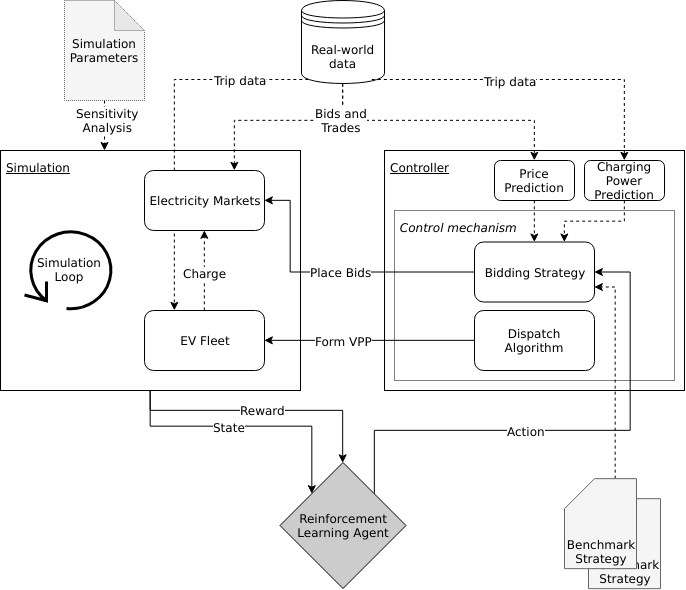
\includegraphics[width=1\linewidth]{./fig/simulation_platform.png}
\caption[FleetSim Architecture]{Architecture of FleetSim \label{fig-fleetsim}}
\end{figure}

\subsection{Modular Expandability}
\label{sec:orgfeae6d3}
\begin{itemize}
\item Plug-in different Market designs
\item Use different real-world data
\item Change Fleet parameters
\item Develop new strategy
\item
\end{itemize}

\clearpage
\section{Results}
\label{sec:org5582d6b}
\subsection{FleetRL}
\label{sec:orgd8ee7f0}
\subsection{Sensitivity Analysis: Prediction Accuracy}
\label{sec:org6f88ce0}
\subsection{Sensitivity Analysis: Infrastructure Changes}
\label{sec:orgeb4e9e3}
\subsection{Sensitivity Analysis: Bidding Strategy}
\label{sec:orgcd1ded9}
\section{Conclusion}
\label{sec:orge6dcd52}
\subsection{Contribution}
\label{sec:org0d37b4d}

\subsection{Limitations}
\label{sec:orgc86fffa}
\subsection{Future Research}
\label{sec:org9f61762}


\clearpage
\bibliography{bibliography/references}
\bibliographystyle{apacite}
\end{document}
